\documentclass[a4paper, 11pt]{article}

\usepackage{fullpage}
%\usepackage[inline]{showlabels}
\usepackage{biblatex}
\usepackage{siunitx}
\usepackage{wrapfig}
\usepackage{amsmath}
\usepackage[german]{babel}
\usepackage{gnuplot-lua-tikz}
\usepackage{chemfig}
\usepackage{subcaption}

\newcommand{\andy}{\qty{2.826e-4}{\per\second}}
\newcommand{\ea}{\qty{1.02777e6}{\joule\per\mole}}
\newcommand{\varAAuAA}{aInf}
\newcommand{\varAAuAB}{-3,7}
\newcommand{\varAAuAC}{}
\newcommand{\varAAuAD}{}
\newcommand{\varABuAA}{a0}
\newcommand{\varABuAB}{9,59847}
\newcommand{\varABuAC}{8,94034}
\newcommand{\varABuAD}{9,49963}
\newcommand{\varACuAA}{K}
\newcommand{\varACuAB}{0,00013}
\newcommand{\varACuAC}{0,00043}
\newcommand{\varACuAD}{0,00013}
\newcommand{\varADuAA}{Ea}
\newcommand{\varADuAB}{1027,7727217253}
\newcommand{\varADuAC}{}
\newcommand{\varADuAD}{}
\newcommand{\varAEuAA}{A}
\newcommand{\varAEuAB}{0,000282616271635305}
\newcommand{\varAEuAC}{}
\newcommand{\varAEuAD}{}
\newcommand{\varAFuAA}{T0}
\newcommand{\varAFuAB}{3856,32015412672}
\newcommand{\varAFuAC}{}
\newcommand{\varAFuAD}{}
\newcommand{\varAGuAA}{T25}
\newcommand{\varAGuAB}{3712,71975162695}
\newcommand{\varAGuAC}{}
\newcommand{\varAGuAD}{}
\newcommand{\varAHuAA}{T50}
\newcommand{\varAHuAB}{3595,51723222914}
\newcommand{\varAHuAC}{}
\newcommand{\varAHuAD}{}
\newcommand{\varAIuAA}{T100}
\newcommand{\varAIuAB}{3415,85856849857}
\newcommand{\varAIuAC}{}
\newcommand{\varAIuAD}{}


\title{Praktikum der physikalischen Chemie\\\large K1 - Aktivierungsenergie der Inversion von Rohrzucker}
\author{Janosch Ehlers (jaeh@uni-bremen.de)\\Samed Hür (huer@uni-bremen.de)\\\textbf{Betreuerin:} Petra Martinovic (p.martinovic@uni-bremen.de)}
\date{02.12.22}
\bibliography{K1.bib}

\begin{document}
\maketitle
\thispagestyle{empty}
\newpage

\thispagestyle{empty}
\tableofcontents
\newpage
\pagenumbering{arabic}

Ziel des Versuches ist es, die Reaktionsgeschwindigkeitskonstante $k$ und die molare Aktivierungsenergie $E_A$ von der Inversionsreaktion von Rohrzucker (Saccharose) zu bestimmen. 
Mithilfe einer polarimetrischen Messung zur Bestimmung des Drehwinkels. 

\section{Theoretischer Hintergrund}
Die Inversionsreaktion von Rohrzucker (Saccharose) wird durch ein Proton katalysiert. 
Saccharose wird zu Glukose und Fruktose umgesetzt. 
\begin{equation}
\schemestart
\chemname{\chemfig{C_{12}H_{22}O_{11}}}{Saccharose} \arrow{->[$H^+$]}\chemname{\chemfig{C_6H_{12}O_6}}{Glukose} + \chemname{\chemfig{C_6H_{12}O_6}}{Fruktose}
\schemestop
\end{equation}
Die Mischung aus Fruktose und Glukose wird als  Invertzucker bezeichnet. 
Saccharose und der Invertzucker sind optisch aktiv. 
Die äquimolare Mischung von Fruktose und Glukose hat in Summe einen kleineren Drehwinkel als die Saccharose. 
So kann der Reaktionsfortschritt anhand der Verkleinerung des Drehwinkels der Lösung betrachtet werden. 
Saccharose dreht die Ebene nach rechts (positiv) und der Invertzucker nach links (negativ). 
Beim arbeiten mit einer verdünnten wässrigen Lösung kann das Wasser als konstant angesehen werden.
Die Reaktionsgeschwindigkeit $k$ lässt sich mit der Gleichung \ref{eq:ln-alpha} berechnen. 
Der linke Term wird in Abhängigkeit von der Zeit dargestellt.
Die Steigung einer Ausgleichsgerade gibt dann die Reaktionsgeschwindigkeitskonstante.
\begin{equation}
	\ln \left( \frac{\alpha_0 - \alpha_\infty}{\alpha - \alpha_\infty }\right) = k \cdot t 
\label{eq:ln-alpha}
\end{equation}
Der Fehler dieser Darstellung lässt sich über die Gleichung \ref{eq:dLNalpha} berechnen.
\begin{equation}
\Delta \ln \left( \frac{\alpha_0 - \alpha_\infty}{\alpha - \alpha_\infty }\right)  = \sqrt{\left(\frac{\Delta \alpha}{\alpha_0 - \alpha_\infty}\right)^2 +\left(\frac{\Delta \alpha \cdot \left(\alpha_0 -\alpha\right)}{\left(\alpha_\infty - \alpha\right)\cdot \left(\alpha_\infty-\alpha_0\right) }\right)^2 +\left(\frac{\Delta \alpha}{\alpha_\infty - \alpha}\right)^2}  \\
\label{eq:dLNalpha}
\end{equation}
Nach dem Arrhenius-Gesetz lässt sich aus der Änderung der Geschwindigkeitskonstante $k$, mit der Temperatur $T$ die Aktivierungsenergie berechnen, mit:
\begin{equation}
\ln (k) = -\frac{E_A}{R} \cdot \left( \frac{1}{T} \right) + \ln (A) \label{eq:EA}
\end{equation}
In der Darstellung werden dann die Fehlerkreuze benötigt.
Diese werden über die Gleichungen \ref{eq:dLNk} und \ref{eq:d1T} berechnet.
\begin{align}
\Delta \left(\ln (k)\right)&=\sqrt{\left(\frac{\delta \ln (k)}{\delta k}\cdot \Delta k \right)^2} = \frac{\Delta k}{k} \label{eq:dLNk}\\
\Delta \left(\frac{1}{T}\right)&=\sqrt{\left(\frac{\delta \frac{1}{T}}{\delta T}\cdot \Delta T \right)^2} = -\frac{\Delta T}{T^2}\label{eq:d1T}
\end{align}
Der Fehler für die Aktivierungsenergie und der Geschwindigkeitskonstante wird graphisch ermittelt über die Auswertung die Fehlerkreuze. 
Zur Bestimmung der Fehler werden jeweils zwei Extremgeraden eingezeichnet, welche jeweils durch $\frac{2}{3}$ der Fehlerboxen verläuft.
Außerdem wird $t_{1/2}$ mit der Gleichung \ref{eq:t0.5} ermittelt.
\begin{equation}
t_{1/2} = \frac{\ln (2)}{k} = \frac{\ln (2)}{A \cdot e^\frac{-E_A}{R\cdot T}}
\label{eq:t0.5}
\end{equation}
Die Fehler der Halbwertzeiten folgen aus der Fehlerfortpflanzung nach Gleichung \ref{eq:dt05}
\begin{align}
\Delta t_{1/2} &= \sqrt{\left(\frac{\delta t_{1/2}}{\delta A}\cdot \Delta A\right)^2 + \left(\frac{\delta t_{1/2}}{\delta E_A}\cdot \Delta E_A\right)^2 +\left(\frac{\delta t_{1/2}}{\delta T}\cdot \Delta T \right)^2}\\
\frac{\delta t_{1/2}}{\delta A} &= - \frac{1}{A^2} \cdot \frac{\ln (2)}{e^{- \frac{E_A}{R \cdot T}}}\\
\frac{\delta t_{1/2}}{\delta E_A} &= \frac{\ln (2)}{A\cdot R \cdot T\cdot e^{\left(- \frac{E_A}{R \cdot T}\right)}} \\
\frac{\delta t_{1/2}}{\delta T} &= - \frac{E_A}{R\cdot T^2}\cdot \frac{\ln (2)}{A\cdot e^{\left(- \frac{E_A}{R \cdot T}\right)}}\\
\Rightarrow \Delta t_{1/2} &= \sqrt{\left(\frac{\ln (2)}{A\cdot e^{- \left(\frac{E_A}{R\cdot T}\right)}}\right)^2 \cdot \left(\left(\frac{\Delta A}{A}\right)^2 + \left(\frac{\Delta E_A}{R\cdot  T}\right)^2 + \left(\frac{E_A \cdot \Delta T}{R\cdot T^2}\right)^2\right)}
\end{align}

\section{Durchführung}
Der Thermostat war schon vor dem Versuch eingeschaltet und auf \qty{25}{\degreeCelsius} eingestellt. 
Danach wurde der Nullpunkt des Polarimeters mit destilliertem Wasser kontrolliert. 
So soll der Größtfehler des Polarimeters abgeschätzt werden.
Anschließend wurden etwa \qty{100}{\milli\liter} einer Rohrzuckerlösung und etwa \qty{100}{\milli\liter} einer HCL-Lösung abgefüllt und unabhängig voneinander im Wasserbad auf \qty{25}{\degreeCelsius} temperiert. 
Dann wurden jeweils \qty{25}{\milli\liter} der HCL-Lösung und der Rohrzuckerlösung in einem Becherglas vermischt. 
Gleichzeitig wurde die Zeitmessung gestartet. 
Danach wurde rasch mit einer Pipette genug Flüssigkeit von der Mischung entnommen, um das Polarimeterrohr blasenfrei zu befüllen. 
Eine Messung dauerte \qty{20}{\minute}, dabei wurden in den ersten \qty{10}{\minute} alle \qty{30}{\second} abgelesen und danach alle \qty{60}{\second}. 
Die Messungen wurden für \qty{30}{\degreeCelsius} und \qty{35}{\degreeCelsius} wiederholt. 
Für die Messung von $\alpha_\infty$ wurde zuerst \qty{25}{\milli\liter} der Messlösung  im Wasserbad auf \qty{70}{\degreeCelsius} erhitzt und anschließend auf \qty{20}{\degreeCelsius} abgekühlt. 
Danach wurde das Polarimeter blasenfrei mit der Messlösung gefüllt und der Wert für $\alpha_\infty$ abgelesen.


\newpage
\begin{wraptable}{l}{0.3\linewidth}
	\begin{tabular}{l|ccc}
		\hline
		t / s & $\alpha_{25}$ & $\alpha_{30}$ & $\alpha_{35}$\\
		\hline
		\hline
5       & -               & -               & -\\
35      & -               & -               & -\\
65      & -               & -               & -\\
95      & 9,55            & -               & -\\
125     & 9,05            & -               & -\\
155     & 9,05            & -               & 9,1\\
185     & 9,25            & 8,85            & 8,95\\
215     & 9,15            & 8,6             & 8,6\\
245     & 9,1             & 8,4             & 8,2\\
275     & 9,15            & 8,1             & 7,85\\
305     & 9,05            & 8               & 7,85\\
335     & 8,95            & 7,8             & 7,6\\
365     & 8,9             & 7,6             & 7,3\\
395     & 8,9             & 7,3             & 7,15\\
425     & 8,8             & 7,6             & 6,9\\
455     & 8,75            & 7,5             & 6,55\\
485     & 8,7             & 7,3             & 6,3\\
515     & 8,5             & 7,3             & 6,2\\
545     & 8,55            & 6,7             & 6\\
575     & 8,45            & 6,65            & 5,65\\
605     & 8,4             & 6,35            & 5,4\\
635     & 8,25            & 6,55            & 5,25\\
665     & 8,25            & 6,35            & 5,15\\
695     & 8,2             & 6,05            & 4,95\\
725     & -               & 6,5             & 4,65\\
755     & 7,95            & 6,05            & -\\
785     & -               & -               & 4,45\\
815     & 7,95            & 5,9             & -\\
845     & -               & -               & 4,2\\
875     & 7,8             & 5,75            & -\\
905     & -               & -               & 3,95\\
935     & 7,8             & 5,45            & -\\
965     & -               & -               & 3,8\\
995     & 7,5             & 5               & -\\
1025    & -               & -               & 3,25\\
1055    & 7,55            & 5,35            & -\\
1085    & -               & -               & 3\\
1115    & 7,25            & 5,25            & -\\
1145    & -               & -               & 2,85\\
1175    & 7,2             & 5,1             & -\\
1205    & -               & -               & 2,5\\
1235    & 7               & 4,95            & -\\
1265    & -               & -               & 2,05\\
1295    & 6,95            & 4,8             & -\\
1325    & -               & -               & 1,95\\
1355    & 6,9             & 4,5             & -\\
1385    & -               & -               & 1,7\\
1415    & -               & 4,4             & -\\
		\hline
	\end{tabular}
	\caption{Drehwinkel über Zeit bei verschiedenen Temperaturen}
	\label{tab:Rohdaten}
\end{wraptable}

\section{Auswertung}
$\alpha_\infty$ spiegelt in unserem Versuch den Drehwinkel wieder, bei dem die Reaktion vollständig abgelaufen ist.
Nach unserer Methode wurde ein Wert von \qty{-3,7}{\degree} bestimmt.
Die Messung der Drehwinkel bei den verschiedenen Temperaturen ergab die in Tabelle \ref{tab:Rohdaten} dargestellten Werte.
Visualisiert ist hier der Drehwinkel ($\alpha$) zu verschiedenen Zeitpunkten der Reaktionen.
Außerdem ist der Drehwinkel in Abhängigkeit der Zeit in der Abbildung \ref{abb:Rohdaten} dargestellt.
Dessen Linearregression gibt über den Y-Achsenabschnitt den extrapolierten Anfangsdrehwinkel.
Daraus ergibt sich ein $\alpha_{0(T_{25})} = \qty{9,6}{\degree}$,$\alpha_{0(T_{30})} = \qty{8,9}{\degree}$ und $\alpha_{0(T_{35})} = \qty{9,4}{\degree}$.
Über Gleichung \ref{eq:ln-alpha} verrechnen wir die bereits erhaltenen Konstanten mit den Rohdaten. Diese werden dann in Abhängigkeit der Zeit dargestellt (Abbildungen \ref{abb:e25}, \ref{abb:e30} und \ref{abb:e35}). 
Beispielhaft ist für 
$\alpha_{25}=\qty{9,55}{\degree}$,
$\alpha_{\infty}=\qty{-3,7}{\degree}$, 
$\alpha_0=\qty{9,6}{\degree}$ 
und $t=90\ s$ nach Gleichung \ref{eq:ln-alpha}, der linke Term ausgerechnet.
Dieser Wert wurde dann in Abbildung \ref{abb:e35} bei $90\ s$ eingetragen. 
Analog wurde mit den anderen Werten verfahren.
 
\begin{equation}
	\ln \left( \frac{\qty{9.59}{\degree} -( \qty{-3.7}{\degree})}{\qty{9.55}{\degree} - (\qty{-3.7}{\degree}) }\right) = \qty{3,014e-3}{}
	\label{eqbsp:ln-aplha}
\end{equation}

Außerdem wird der Drehwinkelfehler mit \qty{0,2}{\degree} und der Zeitfehler mit \qty{5}{\second} bemessen.
Da es immer eine gewisse Zeit braucht, um den Drehwinkel abzulesen, haben wir auf jeden Zeitwert 5\ s addiert. 
Mit dem angegeben Fehlerwert ergibt sich ein Fehlerbereich von 0 bis +10\ s  um den eigentlichen Messwert herum.
Der eingezeichnete Ordinatenfehler errechnet sich nach \ref{eq:dLNalpha}.
Beispielhaft ist dies, für $\alpha=\ang{9,55} ,\alpha_0=\ang{9,598}, \alpha_\infty=\ang{-3,7}$,  hier dargestellt:
\begin{equation}
\resizebox{0.75\hsize}{!}{$%
\Delta \ln (K) =\\ \sqrt{
        \left(\frac{\qty{0.2}{\degree}}{\qty{9.598}{\degree} - (\qty{- 3.7}{\degree})}\right)^2 +
        \left(\frac{\qty{0.2}{\degree} \cdot \left(\qty{9.598}{\degree} -\qty{9.55}{\degree}\right)}{\left(\qty{- 3.7}{\degree} - \qty{9.55}{\degree}\right)\cdot \left(\qty{- 3.7}{\degree}-\qty{9.598}{\degree} \right) }\right)^2 +
        \left(\frac{\qty{0.2}{\degree}}{\qty{- 3.7}{\degree} - \qty{9,55}{\degree}}\right)^2 
        } = 0.021$%
}%
\end{equation}
Mit den Fehlerkreuzen konnten nun die Extremgeraden bestimmen werden.
Diese sollen $\frac{2}{3}$ aller Fehlerbereiche schneiden.
In Tabelle \ref{tab:eqnarray} sind die Gleichungen der Extremgeraden und Ausgleichsgeraden dargestellt.
Nach Gleichung \ref{eq:EA} wird die logarithmische Reaktionsgeschwindigkeit ($k$) in Abhängigkeit von der reziproken Temperatur ($1/T$) dargestellt. 
Über diesen Datensatz wird eine lineare Regression gelegt.
Die Steigung ist nach Gleichung \ref{eq:EA} gleichzusetzen mit $\frac{-E_A}{R}$.
Der Y-Achsenabschnitt ist dann gleich $\ln{(A)}$.
Dargestellt ist dies in Abbildung \ref{abb:EA}.

\begin{equation}
	t_{1/2} = \frac{\ln (2)}{\qty{1.85e15}{\per\second} \cdot exp\left(\frac{-\qty{108576,99}{\joule\per\mole}}{8.3144\frac{J}{mol\cdot K}\cdot 298.14\ K}\right)}= \qty{3928,88}{\second}
\label{eqbsp:t0.5}
\end{equation}

\newpage
\clearpage

Zuletzt wird über die errechneten Daten die Halbwertszeiten der Reaktion von den Temperaturen \qty{0}{\degreeCelsius}, \qty{25}{\degreeCelsius}, \qty{50}{\degreeCelsius} und \qty{100}{\degreeCelsius} berechnet.
Genutzt wird hierfür Gleichung \ref{eq:t0.5}.
Beispielhaft für $T=273.14\ K$ ist die Halbwertszeit in Gleichung \ref{eqbsp:t0.5} berechnet.
Der Fehler der Halbwertszeit wird nach Gleichung \ref{eqbsp:dt05} berechnet.
$\Delta A$ berechnet sich aus der Mittelwertabweichung der Ordinatenabschnitte der Extremgeraden.
Während $\Delta E_A$ die Mittelwertabweichung der Steigungen der Extremgeraden, geteilt durch die ideale Gaskonstante ist.
Beispielhaft ist dies für $T=273.14\ K$, $E_A=\qty{108576,99}{\joule\per\mole}$ und $A=\qty{1,85e15}{\per\second}$ im Folgenden gezeigt:
\begin{eqnarray*}
\Delta t_{1/2} =\\
\resizebox{\hsize}{!}{$%
\sqrt{\left(\frac{\ln (2)}{\qty{1,85e15}{\per\second}\cdot e^{- \left(\frac{\qty{108576,99}{\joule\per\mole}}{\qty{8,31446}{\joule\per\mole\per\kelvin}\cdot \qty{273,14}{\kelvin}}\right)}}\right)^2 \cdot \left(\left(\frac{\qty{13,2}{\per\second}}{\qty{1,85e15}{\per\second}}\right)^2 + \left(\frac{\qty{962,17}{\joule\per\mole}}{\qty{8,314}{\joule\per\mole\per\kelvin}\cdot  \qty{273,14}{\kelvin}}\right)^2 + \left(\frac{\qty{108576,99}{\joule\per\mole} \cdot\qty{1,126}{\kelvin}}{\qty{8,314}{\joule\per\mole\per\kelvin}\cdot (\qty{273,14}{\kelvin})^2}\right)^2\right)}
$%
}% 
\\= \qty{-1,125e-6}{\second}
\end{eqnarray*}
\begin{table}[t]
	\centering
	\begin{tabular}{l|lll}
		\hline
		$T$ 				& obere Extremgerade		& Ausgleichsgerade	& untere Extremgerade\\
		\hline
		\hline
		\qty{25}{\degreeCelsius} 	& $0,00024x-0,0426$ 		& $0,00018x-0,0066$	& $0,00011x+0,0351$\\
		\qty{30}{\degreeCelsius}	& $0,00041x-0,0522$ 		& $0,00037x-0,0302$ 	& $0,00032x+0$\\
		\qty{35}{\degreeCelsius}	& $0,00081x-0,1360$ 		& $0,00073x-0,0840$ 	& $0,00065x-0,029$\\
		\hline
	\end{tabular}
	\caption{Geradengleichungen der Reaktionsgeschwindigkeitskonstanten Bestimmung}
	\label{tab:eqnarray}
\end{table}


\begin{figure}
\centering
	\begin{subfigure}{0.4\textwidth}
	\begin{tikzpicture}[gnuplot, scale=0.5, every node/.style={scale=0.5}]
%% generated with GNUPLOT 5.4p5 (Lua 5.4; terminal rev. Jun 2020, script rev. 115)
%% Fr 02 Dez 2022 17:37:53 CET
\path (0.000,0.000) rectangle (12.500,8.750);
\gpcolor{color=gp lt color border}
\gpsetlinetype{gp lt border}
\gpsetdashtype{gp dt solid}
\gpsetlinewidth{1.00}
\draw[gp path] (1.380,0.985)--(1.560,0.985);
\draw[gp path] (11.947,0.985)--(11.767,0.985);
\node[gp node right] at (1.196,0.985) {$-0.05$};
\draw[gp path] (1.380,2.050)--(1.560,2.050);
\draw[gp path] (11.947,2.050)--(11.767,2.050);
\node[gp node right] at (1.196,2.050) {$0$};
\draw[gp path] (1.380,3.115)--(1.560,3.115);
\draw[gp path] (11.947,3.115)--(11.767,3.115);
\node[gp node right] at (1.196,3.115) {$0.05$};
\draw[gp path] (1.380,4.180)--(1.560,4.180);
\draw[gp path] (11.947,4.180)--(11.767,4.180);
\node[gp node right] at (1.196,4.180) {$0.1$};
\draw[gp path] (1.380,5.246)--(1.560,5.246);
\draw[gp path] (11.947,5.246)--(11.767,5.246);
\node[gp node right] at (1.196,5.246) {$0.15$};
\draw[gp path] (1.380,6.311)--(1.560,6.311);
\draw[gp path] (11.947,6.311)--(11.767,6.311);
\node[gp node right] at (1.196,6.311) {$0.2$};
\draw[gp path] (1.380,7.376)--(1.560,7.376);
\draw[gp path] (11.947,7.376)--(11.767,7.376);
\node[gp node right] at (1.196,7.376) {$0.25$};
\draw[gp path] (1.380,8.441)--(1.560,8.441);
\draw[gp path] (11.947,8.441)--(11.767,8.441);
\node[gp node right] at (1.196,8.441) {$0.3$};
\draw[gp path] (1.380,0.985)--(1.380,1.165);
\draw[gp path] (1.380,8.441)--(1.380,8.261);
\node[gp node center] at (1.380,0.677) {$0$};
\draw[gp path] (2.890,0.985)--(2.890,1.165);
\draw[gp path] (2.890,8.441)--(2.890,8.261);
\node[gp node center] at (2.890,0.677) {$200$};
\draw[gp path] (4.399,0.985)--(4.399,1.165);
\draw[gp path] (4.399,8.441)--(4.399,8.261);
\node[gp node center] at (4.399,0.677) {$400$};
\draw[gp path] (5.909,0.985)--(5.909,1.165);
\draw[gp path] (5.909,8.441)--(5.909,8.261);
\node[gp node center] at (5.909,0.677) {$600$};
\draw[gp path] (7.418,0.985)--(7.418,1.165);
\draw[gp path] (7.418,8.441)--(7.418,8.261);
\node[gp node center] at (7.418,0.677) {$800$};
\draw[gp path] (8.928,0.985)--(8.928,1.165);
\draw[gp path] (8.928,8.441)--(8.928,8.261);
\node[gp node center] at (8.928,0.677) {$1000$};
\draw[gp path] (10.437,0.985)--(10.437,1.165);
\draw[gp path] (10.437,8.441)--(10.437,8.261);
\node[gp node center] at (10.437,0.677) {$1200$};
\draw[gp path] (11.947,0.985)--(11.947,1.165);
\draw[gp path] (11.947,8.441)--(11.947,8.261);
\node[gp node center] at (11.947,0.677) {$1400$};
\draw[gp path] (1.380,8.441)--(1.380,0.985)--(11.947,0.985)--(11.947,8.441)--cycle;
\node[gp node center] at (6.663,0.215) {t / s};
\node[gp node right] at (7.769,8.107) {$25^\circ$};
\gpcolor{rgb color={0.580,0.000,0.827}}
\draw[gp path] (7.953,8.107)--(8.869,8.107);
\draw[gp path] (7.953,8.197)--(7.953,8.017);
\draw[gp path] (8.869,8.197)--(8.869,8.017);
\draw[gp path] (2.059,1.674)--(2.059,2.582);
\draw[gp path] (1.969,1.674)--(2.149,1.674);
\draw[gp path] (1.969,2.582)--(2.149,2.582);
\draw[gp path] (2.286,2.484)--(2.286,3.411);
\draw[gp path] (2.196,2.484)--(2.376,2.484);
\draw[gp path] (2.196,3.411)--(2.376,3.411);
\draw[gp path] (2.512,2.484)--(2.512,3.411);
\draw[gp path] (2.422,2.484)--(2.602,2.484);
\draw[gp path] (2.422,3.411)--(2.602,3.411);
\draw[gp path] (2.739,2.156)--(2.739,3.075);
\draw[gp path] (2.649,2.156)--(2.829,2.156);
\draw[gp path] (2.649,3.075)--(2.829,3.075);
\draw[gp path] (2.965,2.320)--(2.965,3.242);
\draw[gp path] (2.875,2.320)--(3.055,2.320);
\draw[gp path] (2.875,3.242)--(3.055,3.242);
\draw[gp path] (3.191,2.402)--(3.191,3.326);
\draw[gp path] (3.101,2.402)--(3.281,2.402);
\draw[gp path] (3.101,3.326)--(3.281,3.326);
\draw[gp path] (3.418,2.320)--(3.418,3.242);
\draw[gp path] (3.328,2.320)--(3.508,2.320);
\draw[gp path] (3.328,3.242)--(3.508,3.242);
\draw[gp path] (3.644,2.484)--(3.644,3.411);
\draw[gp path] (3.554,2.484)--(3.734,2.484);
\draw[gp path] (3.554,3.411)--(3.734,3.411);
\draw[gp path] (3.871,2.650)--(3.871,3.580);
\draw[gp path] (3.781,2.650)--(3.961,2.650);
\draw[gp path] (3.781,3.580)--(3.961,3.580);
\draw[gp path] (4.097,2.733)--(4.097,3.666);
\draw[gp path] (4.007,2.733)--(4.187,2.733);
\draw[gp path] (4.007,3.666)--(4.187,3.666);
\draw[gp path] (4.324,2.733)--(4.324,3.666);
\draw[gp path] (4.234,2.733)--(4.414,2.733);
\draw[gp path] (4.234,3.666)--(4.414,3.666);
\draw[gp path] (4.550,2.901)--(4.550,3.837);
\draw[gp path] (4.460,2.901)--(4.640,2.901);
\draw[gp path] (4.460,3.837)--(4.640,3.837);
\draw[gp path] (4.777,2.985)--(4.777,3.924);
\draw[gp path] (4.687,2.985)--(4.867,2.985);
\draw[gp path] (4.687,3.924)--(4.867,3.924);
\draw[gp path] (5.003,3.070)--(5.003,4.011);
\draw[gp path] (4.913,3.070)--(5.093,3.070);
\draw[gp path] (4.913,4.011)--(5.093,4.011);
\draw[gp path] (5.229,3.412)--(5.229,4.362);
\draw[gp path] (5.139,3.412)--(5.319,3.412);
\draw[gp path] (5.139,4.362)--(5.319,4.362);
\draw[gp path] (5.456,3.326)--(5.456,4.273);
\draw[gp path] (5.366,3.326)--(5.546,3.326);
\draw[gp path] (5.366,4.273)--(5.546,4.273);
\draw[gp path] (5.682,3.498)--(5.682,4.450);
\draw[gp path] (5.592,3.498)--(5.772,3.498);
\draw[gp path] (5.592,4.450)--(5.772,4.450);
\draw[gp path] (5.909,3.585)--(5.909,4.539);
\draw[gp path] (5.819,3.585)--(5.999,3.585);
\draw[gp path] (5.819,4.539)--(5.999,4.539);
\draw[gp path] (6.135,3.847)--(6.135,4.808);
\draw[gp path] (6.045,3.847)--(6.225,3.847);
\draw[gp path] (6.045,4.808)--(6.225,4.808);
\draw[gp path] (6.362,3.847)--(6.362,4.808);
\draw[gp path] (6.272,3.847)--(6.452,3.847);
\draw[gp path] (6.272,4.808)--(6.452,4.808);
\draw[gp path] (6.588,3.935)--(6.588,4.899);
\draw[gp path] (6.498,3.935)--(6.678,3.935);
\draw[gp path] (6.498,4.899)--(6.678,4.899);
\draw[gp path] (7.041,4.381)--(7.041,5.358);
\draw[gp path] (6.951,4.381)--(7.131,4.381);
\draw[gp path] (6.951,5.358)--(7.131,5.358);
\draw[gp path] (7.494,4.381)--(7.494,5.358);
\draw[gp path] (7.404,4.381)--(7.584,4.381);
\draw[gp path] (7.404,5.358)--(7.584,5.358);
\draw[gp path] (7.947,4.653)--(7.947,5.638);
\draw[gp path] (7.857,4.653)--(8.037,4.653);
\draw[gp path] (7.857,5.638)--(8.037,5.638);
\draw[gp path] (8.400,4.653)--(8.400,5.638);
\draw[gp path] (8.310,4.653)--(8.490,4.653);
\draw[gp path] (8.310,5.638)--(8.490,5.638);
\draw[gp path] (8.852,5.208)--(8.852,6.210);
\draw[gp path] (8.762,5.208)--(8.942,5.208);
\draw[gp path] (8.762,6.210)--(8.942,6.210);
\draw[gp path] (9.305,5.114)--(9.305,6.113);
\draw[gp path] (9.215,5.114)--(9.395,5.114);
\draw[gp path] (9.215,6.113)--(9.395,6.113);
\draw[gp path] (9.758,5.681)--(9.758,6.698);
\draw[gp path] (9.668,5.681)--(9.848,5.681);
\draw[gp path] (9.668,6.698)--(9.848,6.698);
\draw[gp path] (10.211,5.777)--(10.211,6.797);
\draw[gp path] (10.121,5.777)--(10.301,5.777);
\draw[gp path] (10.121,6.797)--(10.301,6.797);
\draw[gp path] (10.664,6.165)--(10.664,7.198);
\draw[gp path] (10.574,6.165)--(10.754,6.165);
\draw[gp path] (10.574,7.198)--(10.754,7.198);
\draw[gp path] (11.117,6.263)--(11.117,7.300);
\draw[gp path] (11.027,6.263)--(11.207,6.263);
\draw[gp path] (11.027,7.300)--(11.207,7.300);
\draw[gp path] (2.022,2.128)--(2.097,2.128);
\draw[gp path] (2.022,2.038)--(2.022,2.218);
\draw[gp path] (2.097,2.038)--(2.097,2.218);
\draw[gp path] (2.248,2.947)--(2.323,2.947);
\draw[gp path] (2.248,2.857)--(2.248,3.037);
\draw[gp path] (2.323,2.857)--(2.323,3.037);
\draw[gp path] (2.474,2.947)--(2.550,2.947);
\draw[gp path] (2.474,2.857)--(2.474,3.037);
\draw[gp path] (2.550,2.857)--(2.550,3.037);
\draw[gp path] (2.701,2.616)--(2.776,2.616);
\draw[gp path] (2.701,2.526)--(2.701,2.706);
\draw[gp path] (2.776,2.526)--(2.776,2.706);
\draw[gp path] (2.927,2.781)--(3.003,2.781);
\draw[gp path] (2.927,2.691)--(2.927,2.871);
\draw[gp path] (3.003,2.691)--(3.003,2.871);
\draw[gp path] (3.154,2.864)--(3.229,2.864);
\draw[gp path] (3.154,2.774)--(3.154,2.954);
\draw[gp path] (3.229,2.774)--(3.229,2.954);
\draw[gp path] (3.380,2.781)--(3.456,2.781);
\draw[gp path] (3.380,2.691)--(3.380,2.871);
\draw[gp path] (3.456,2.691)--(3.456,2.871);
\draw[gp path] (3.607,2.947)--(3.682,2.947);
\draw[gp path] (3.607,2.857)--(3.607,3.037);
\draw[gp path] (3.682,2.857)--(3.682,3.037);
\draw[gp path] (3.833,3.115)--(3.909,3.115);
\draw[gp path] (3.833,3.025)--(3.833,3.205);
\draw[gp path] (3.909,3.025)--(3.909,3.205);
\draw[gp path] (4.059,3.199)--(4.135,3.199);
\draw[gp path] (4.059,3.109)--(4.059,3.289);
\draw[gp path] (4.135,3.109)--(4.135,3.289);
\draw[gp path] (4.286,3.199)--(4.361,3.199);
\draw[gp path] (4.286,3.109)--(4.286,3.289);
\draw[gp path] (4.361,3.109)--(4.361,3.289);
\draw[gp path] (4.512,3.369)--(4.588,3.369);
\draw[gp path] (4.512,3.279)--(4.512,3.459);
\draw[gp path] (4.588,3.279)--(4.588,3.459);
\draw[gp path] (4.739,3.455)--(4.814,3.455);
\draw[gp path] (4.739,3.365)--(4.739,3.545);
\draw[gp path] (4.814,3.365)--(4.814,3.545);
\draw[gp path] (4.965,3.540)--(5.041,3.540);
\draw[gp path] (4.965,3.450)--(4.965,3.630);
\draw[gp path] (5.041,3.450)--(5.041,3.630);
\draw[gp path] (5.192,3.887)--(5.267,3.887);
\draw[gp path] (5.192,3.797)--(5.192,3.977);
\draw[gp path] (5.267,3.797)--(5.267,3.977);
\draw[gp path] (5.418,3.800)--(5.494,3.800);
\draw[gp path] (5.418,3.710)--(5.418,3.890);
\draw[gp path] (5.494,3.710)--(5.494,3.890);
\draw[gp path] (5.645,3.974)--(5.720,3.974);
\draw[gp path] (5.645,3.884)--(5.645,4.064);
\draw[gp path] (5.720,3.884)--(5.720,4.064);
\draw[gp path] (5.871,4.062)--(5.946,4.062);
\draw[gp path] (5.871,3.972)--(5.871,4.152);
\draw[gp path] (5.946,3.972)--(5.946,4.152);
\draw[gp path] (6.097,4.328)--(6.173,4.328);
\draw[gp path] (6.097,4.238)--(6.097,4.418);
\draw[gp path] (6.173,4.238)--(6.173,4.418);
\draw[gp path] (6.324,4.328)--(6.399,4.328);
\draw[gp path] (6.324,4.238)--(6.324,4.418);
\draw[gp path] (6.399,4.238)--(6.399,4.418);
\draw[gp path] (6.550,4.417)--(6.626,4.417);
\draw[gp path] (6.550,4.327)--(6.550,4.507);
\draw[gp path] (6.626,4.327)--(6.626,4.507);
\draw[gp path] (7.003,4.869)--(7.079,4.869);
\draw[gp path] (7.003,4.779)--(7.003,4.959);
\draw[gp path] (7.079,4.779)--(7.079,4.959);
\draw[gp path] (7.456,4.869)--(7.532,4.869);
\draw[gp path] (7.456,4.779)--(7.456,4.959);
\draw[gp path] (7.532,4.779)--(7.532,4.959);
\draw[gp path] (7.909,5.145)--(7.984,5.145);
\draw[gp path] (7.909,5.055)--(7.909,5.235);
\draw[gp path] (7.984,5.055)--(7.984,5.235);
\draw[gp path] (8.362,5.145)--(8.437,5.145);
\draw[gp path] (8.362,5.055)--(8.362,5.235);
\draw[gp path] (8.437,5.055)--(8.437,5.235);
\draw[gp path] (8.815,5.709)--(8.890,5.709);
\draw[gp path] (8.815,5.619)--(8.815,5.799);
\draw[gp path] (8.890,5.619)--(8.890,5.799);
\draw[gp path] (9.268,5.614)--(9.343,5.614);
\draw[gp path] (9.268,5.524)--(9.268,5.704);
\draw[gp path] (9.343,5.524)--(9.343,5.704);
\draw[gp path] (9.720,6.189)--(9.796,6.189);
\draw[gp path] (9.720,6.099)--(9.720,6.279);
\draw[gp path] (9.796,6.099)--(9.796,6.279);
\draw[gp path] (10.173,6.287)--(10.249,6.287);
\draw[gp path] (10.173,6.197)--(10.173,6.377);
\draw[gp path] (10.249,6.197)--(10.249,6.377);
\draw[gp path] (10.626,6.681)--(10.702,6.681);
\draw[gp path] (10.626,6.591)--(10.626,6.771);
\draw[gp path] (10.702,6.591)--(10.702,6.771);
\draw[gp path] (11.079,6.781)--(11.154,6.781);
\draw[gp path] (11.079,6.691)--(11.079,6.871);
\draw[gp path] (11.154,6.691)--(11.154,6.871);
\gpsetpointsize{4.00}
\gp3point{gp mark 1}{}{(2.059,2.128)}
\gp3point{gp mark 1}{}{(2.286,2.947)}
\gp3point{gp mark 1}{}{(2.512,2.947)}
\gp3point{gp mark 1}{}{(2.739,2.616)}
\gp3point{gp mark 1}{}{(2.965,2.781)}
\gp3point{gp mark 1}{}{(3.191,2.864)}
\gp3point{gp mark 1}{}{(3.418,2.781)}
\gp3point{gp mark 1}{}{(3.644,2.947)}
\gp3point{gp mark 1}{}{(3.871,3.115)}
\gp3point{gp mark 1}{}{(4.097,3.199)}
\gp3point{gp mark 1}{}{(4.324,3.199)}
\gp3point{gp mark 1}{}{(4.550,3.369)}
\gp3point{gp mark 1}{}{(4.777,3.455)}
\gp3point{gp mark 1}{}{(5.003,3.540)}
\gp3point{gp mark 1}{}{(5.229,3.887)}
\gp3point{gp mark 1}{}{(5.456,3.800)}
\gp3point{gp mark 1}{}{(5.682,3.974)}
\gp3point{gp mark 1}{}{(5.909,4.062)}
\gp3point{gp mark 1}{}{(6.135,4.328)}
\gp3point{gp mark 1}{}{(6.362,4.328)}
\gp3point{gp mark 1}{}{(6.588,4.417)}
\gp3point{gp mark 1}{}{(7.041,4.869)}
\gp3point{gp mark 1}{}{(7.494,4.869)}
\gp3point{gp mark 1}{}{(7.947,5.145)}
\gp3point{gp mark 1}{}{(8.400,5.145)}
\gp3point{gp mark 1}{}{(8.852,5.709)}
\gp3point{gp mark 1}{}{(9.305,5.614)}
\gp3point{gp mark 1}{}{(9.758,6.189)}
\gp3point{gp mark 1}{}{(10.211,6.287)}
\gp3point{gp mark 1}{}{(10.664,6.681)}
\gp3point{gp mark 1}{}{(11.117,6.781)}
\gp3point{gp mark 1}{}{(8.411,8.107)}
\gpcolor{color=gp lt color border}
\node[gp node right] at (7.769,7.799) {Obere Extremgerade};
\gpcolor{rgb color={0.000,0.620,0.451}}
\draw[gp path] (7.953,7.799)--(8.869,7.799);
\draw[gp path] (2.022,1.578)--(2.114,1.641)--(2.206,1.703)--(2.298,1.766)--(2.391,1.828)%
  --(2.483,1.891)--(2.575,1.953)--(2.667,2.016)--(2.760,2.078)--(2.852,2.141)--(2.944,2.203)%
  --(3.036,2.266)--(3.129,2.328)--(3.221,2.391)--(3.313,2.453)--(3.405,2.516)--(3.498,2.578)%
  --(3.590,2.641)--(3.682,2.703)--(3.774,2.766)--(3.867,2.828)--(3.959,2.891)--(4.051,2.953)%
  --(4.143,3.016)--(4.236,3.078)--(4.328,3.140)--(4.420,3.203)--(4.512,3.265)--(4.605,3.328)%
  --(4.697,3.390)--(4.789,3.453)--(4.881,3.515)--(4.974,3.578)--(5.066,3.640)--(5.158,3.703)%
  --(5.250,3.765)--(5.343,3.828)--(5.435,3.890)--(5.527,3.953)--(5.619,4.015)--(5.712,4.078)%
  --(5.804,4.140)--(5.896,4.203)--(5.988,4.265)--(6.081,4.328)--(6.173,4.390)--(6.265,4.453)%
  --(6.357,4.515)--(6.450,4.578)--(6.542,4.640)--(6.634,4.703)--(6.726,4.765)--(6.819,4.828)%
  --(6.911,4.890)--(7.003,4.953)--(7.095,5.015)--(7.188,5.078)--(7.280,5.140)--(7.372,5.203)%
  --(7.464,5.265)--(7.557,5.328)--(7.649,5.390)--(7.741,5.453)--(7.833,5.515)--(7.926,5.578)%
  --(8.018,5.640)--(8.110,5.703)--(8.202,5.765)--(8.295,5.827)--(8.387,5.890)--(8.479,5.952)%
  --(8.571,6.015)--(8.664,6.077)--(8.756,6.140)--(8.848,6.202)--(8.940,6.265)--(9.033,6.327)%
  --(9.125,6.390)--(9.217,6.452)--(9.309,6.515)--(9.402,6.577)--(9.494,6.640)--(9.586,6.702)%
  --(9.678,6.765)--(9.771,6.827)--(9.863,6.890)--(9.955,6.952)--(10.047,7.015)--(10.140,7.077)%
  --(10.232,7.140)--(10.324,7.202)--(10.416,7.265)--(10.509,7.327)--(10.601,7.390)--(10.693,7.452)%
  --(10.785,7.515)--(10.878,7.577)--(10.970,7.640)--(11.062,7.702)--(11.154,7.765);
\gpcolor{color=gp lt color border}
\node[gp node right] at (7.769,7.491) {Ausgleichsgerade};
\gpcolor{rgb color={0.337,0.706,0.914}}
\draw[gp path] (7.953,7.491)--(8.869,7.491);
\draw[gp path] (2.022,2.235)--(2.114,2.282)--(2.206,2.329)--(2.298,2.376)--(2.391,2.423)%
  --(2.483,2.470)--(2.575,2.517)--(2.667,2.564)--(2.760,2.610)--(2.852,2.657)--(2.944,2.704)%
  --(3.036,2.751)--(3.129,2.798)--(3.221,2.845)--(3.313,2.892)--(3.405,2.938)--(3.498,2.985)%
  --(3.590,3.032)--(3.682,3.079)--(3.774,3.126)--(3.867,3.173)--(3.959,3.220)--(4.051,3.267)%
  --(4.143,3.313)--(4.236,3.360)--(4.328,3.407)--(4.420,3.454)--(4.512,3.501)--(4.605,3.548)%
  --(4.697,3.595)--(4.789,3.641)--(4.881,3.688)--(4.974,3.735)--(5.066,3.782)--(5.158,3.829)%
  --(5.250,3.876)--(5.343,3.923)--(5.435,3.970)--(5.527,4.016)--(5.619,4.063)--(5.712,4.110)%
  --(5.804,4.157)--(5.896,4.204)--(5.988,4.251)--(6.081,4.298)--(6.173,4.344)--(6.265,4.391)%
  --(6.357,4.438)--(6.450,4.485)--(6.542,4.532)--(6.634,4.579)--(6.726,4.626)--(6.819,4.673)%
  --(6.911,4.719)--(7.003,4.766)--(7.095,4.813)--(7.188,4.860)--(7.280,4.907)--(7.372,4.954)%
  --(7.464,5.001)--(7.557,5.047)--(7.649,5.094)--(7.741,5.141)--(7.833,5.188)--(7.926,5.235)%
  --(8.018,5.282)--(8.110,5.329)--(8.202,5.376)--(8.295,5.422)--(8.387,5.469)--(8.479,5.516)%
  --(8.571,5.563)--(8.664,5.610)--(8.756,5.657)--(8.848,5.704)--(8.940,5.750)--(9.033,5.797)%
  --(9.125,5.844)--(9.217,5.891)--(9.309,5.938)--(9.402,5.985)--(9.494,6.032)--(9.586,6.079)%
  --(9.678,6.125)--(9.771,6.172)--(9.863,6.219)--(9.955,6.266)--(10.047,6.313)--(10.140,6.360)%
  --(10.232,6.407)--(10.324,6.453)--(10.416,6.500)--(10.509,6.547)--(10.601,6.594)--(10.693,6.641)%
  --(10.785,6.688)--(10.878,6.735)--(10.970,6.782)--(11.062,6.828)--(11.154,6.875);
\gpcolor{color=gp lt color border}
\node[gp node right] at (7.769,7.183) {Untere Extremgerade};
\gpcolor{rgb color={0.902,0.624,0.000}}
\draw[gp path] (7.953,7.183)--(8.869,7.183);
\draw[gp path] (2.022,2.997)--(2.114,3.026)--(2.206,3.054)--(2.298,3.083)--(2.391,3.112)%
  --(2.483,3.140)--(2.575,3.169)--(2.667,3.198)--(2.760,3.226)--(2.852,3.255)--(2.944,3.283)%
  --(3.036,3.312)--(3.129,3.341)--(3.221,3.369)--(3.313,3.398)--(3.405,3.427)--(3.498,3.455)%
  --(3.590,3.484)--(3.682,3.513)--(3.774,3.541)--(3.867,3.570)--(3.959,3.599)--(4.051,3.627)%
  --(4.143,3.656)--(4.236,3.684)--(4.328,3.713)--(4.420,3.742)--(4.512,3.770)--(4.605,3.799)%
  --(4.697,3.828)--(4.789,3.856)--(4.881,3.885)--(4.974,3.914)--(5.066,3.942)--(5.158,3.971)%
  --(5.250,3.999)--(5.343,4.028)--(5.435,4.057)--(5.527,4.085)--(5.619,4.114)--(5.712,4.143)%
  --(5.804,4.171)--(5.896,4.200)--(5.988,4.229)--(6.081,4.257)--(6.173,4.286)--(6.265,4.315)%
  --(6.357,4.343)--(6.450,4.372)--(6.542,4.400)--(6.634,4.429)--(6.726,4.458)--(6.819,4.486)%
  --(6.911,4.515)--(7.003,4.544)--(7.095,4.572)--(7.188,4.601)--(7.280,4.630)--(7.372,4.658)%
  --(7.464,4.687)--(7.557,4.715)--(7.649,4.744)--(7.741,4.773)--(7.833,4.801)--(7.926,4.830)%
  --(8.018,4.859)--(8.110,4.887)--(8.202,4.916)--(8.295,4.945)--(8.387,4.973)--(8.479,5.002)%
  --(8.571,5.031)--(8.664,5.059)--(8.756,5.088)--(8.848,5.116)--(8.940,5.145)--(9.033,5.174)%
  --(9.125,5.202)--(9.217,5.231)--(9.309,5.260)--(9.402,5.288)--(9.494,5.317)--(9.586,5.346)%
  --(9.678,5.374)--(9.771,5.403)--(9.863,5.431)--(9.955,5.460)--(10.047,5.489)--(10.140,5.517)%
  --(10.232,5.546)--(10.324,5.575)--(10.416,5.603)--(10.509,5.632)--(10.601,5.661)--(10.693,5.689)%
  --(10.785,5.718)--(10.878,5.747)--(10.970,5.775)--(11.062,5.804)--(11.154,5.832);
\gpcolor{color=gp lt color border}
\draw[gp path] (1.380,8.441)--(1.380,0.985)--(11.947,0.985)--(11.947,8.441)--cycle;
%% coordinates of the plot area
\gpdefrectangularnode{gp plot 1}{\pgfpoint{1.380cm}{0.985cm}}{\pgfpoint{11.947cm}{8.441cm}}
\end{tikzpicture}
%% gnuplot variables

	\caption{Logarithmische Drehwinkel Differenzen, bei $\qty{25}{\degreeCelsius}$}
	\label{abb:e25}
	\end{subfigure}
\hspace{5mm}	
	\begin{subfigure}{0.4\textwidth}
	\begin{tikzpicture}[gnuplot, scale=0.5, every node/.style={scale=0.5}]
%% generated with GNUPLOT 5.4p5 (Lua 5.4; terminal rev. Jun 2020, script rev. 115)
%% Fr 02 Dez 2022 17:37:53 CET
\path (0.000,0.000) rectangle (12.500,8.750);
\gpcolor{color=gp lt color border}
\gpsetlinetype{gp lt border}
\gpsetdashtype{gp dt solid}
\gpsetlinewidth{1.00}
\draw[gp path] (1.196,0.985)--(1.376,0.985);
\draw[gp path] (11.947,0.985)--(11.767,0.985);
\node[gp node right] at (1.012,0.985) {$-0.1$};
\draw[gp path] (1.196,2.050)--(1.376,2.050);
\draw[gp path] (11.947,2.050)--(11.767,2.050);
\node[gp node right] at (1.012,2.050) {$0$};
\draw[gp path] (1.196,3.115)--(1.376,3.115);
\draw[gp path] (11.947,3.115)--(11.767,3.115);
\node[gp node right] at (1.012,3.115) {$0.1$};
\draw[gp path] (1.196,4.180)--(1.376,4.180);
\draw[gp path] (11.947,4.180)--(11.767,4.180);
\node[gp node right] at (1.012,4.180) {$0.2$};
\draw[gp path] (1.196,5.246)--(1.376,5.246);
\draw[gp path] (11.947,5.246)--(11.767,5.246);
\node[gp node right] at (1.012,5.246) {$0.3$};
\draw[gp path] (1.196,6.311)--(1.376,6.311);
\draw[gp path] (11.947,6.311)--(11.767,6.311);
\node[gp node right] at (1.012,6.311) {$0.4$};
\draw[gp path] (1.196,7.376)--(1.376,7.376);
\draw[gp path] (11.947,7.376)--(11.767,7.376);
\node[gp node right] at (1.012,7.376) {$0.5$};
\draw[gp path] (1.196,8.441)--(1.376,8.441);
\draw[gp path] (11.947,8.441)--(11.767,8.441);
\node[gp node right] at (1.012,8.441) {$0.6$};
\draw[gp path] (1.196,0.985)--(1.196,1.165);
\draw[gp path] (1.196,8.441)--(1.196,8.261);
\node[gp node center] at (1.196,0.677) {$0$};
\draw[gp path] (2.732,0.985)--(2.732,1.165);
\draw[gp path] (2.732,8.441)--(2.732,8.261);
\node[gp node center] at (2.732,0.677) {$200$};
\draw[gp path] (4.268,0.985)--(4.268,1.165);
\draw[gp path] (4.268,8.441)--(4.268,8.261);
\node[gp node center] at (4.268,0.677) {$400$};
\draw[gp path] (5.804,0.985)--(5.804,1.165);
\draw[gp path] (5.804,8.441)--(5.804,8.261);
\node[gp node center] at (5.804,0.677) {$600$};
\draw[gp path] (7.339,0.985)--(7.339,1.165);
\draw[gp path] (7.339,8.441)--(7.339,8.261);
\node[gp node center] at (7.339,0.677) {$800$};
\draw[gp path] (8.875,0.985)--(8.875,1.165);
\draw[gp path] (8.875,8.441)--(8.875,8.261);
\node[gp node center] at (8.875,0.677) {$1000$};
\draw[gp path] (10.411,0.985)--(10.411,1.165);
\draw[gp path] (10.411,8.441)--(10.411,8.261);
\node[gp node center] at (10.411,0.677) {$1200$};
\draw[gp path] (11.947,0.985)--(11.947,1.165);
\draw[gp path] (11.947,8.441)--(11.947,8.261);
\node[gp node center] at (11.947,0.677) {$1400$};
\draw[gp path] (1.196,8.441)--(1.196,0.985)--(11.947,0.985)--(11.947,8.441)--cycle;
\node[gp node center] at (6.571,0.215) {t / s};
\node[gp node right] at (7.677,8.107) {$30^\circ$};
\gpcolor{rgb color={0.580,0.000,0.827}}
\draw[gp path] (7.861,8.107)--(8.777,8.107);
\draw[gp path] (7.861,8.197)--(7.861,8.017);
\draw[gp path] (8.777,8.197)--(8.777,8.017);
\draw[gp path] (2.578,1.887)--(2.578,2.366);
\draw[gp path] (2.488,1.887)--(2.668,1.887);
\draw[gp path] (2.488,2.366)--(2.668,2.366);
\draw[gp path] (2.809,2.099)--(2.809,2.583);
\draw[gp path] (2.719,2.099)--(2.899,2.099);
\draw[gp path] (2.719,2.583)--(2.899,2.583);
\draw[gp path] (3.039,2.272)--(3.039,2.759);
\draw[gp path] (2.949,2.272)--(3.129,2.272);
\draw[gp path] (2.949,2.759)--(3.129,2.759);
\draw[gp path] (3.269,2.536)--(3.269,3.030);
\draw[gp path] (3.179,2.536)--(3.359,2.536);
\draw[gp path] (3.179,3.030)--(3.359,3.030);
\draw[gp path] (3.500,2.625)--(3.500,3.122);
\draw[gp path] (3.410,2.625)--(3.590,2.625);
\draw[gp path] (3.410,3.122)--(3.590,3.122);
\draw[gp path] (3.730,2.806)--(3.730,3.308);
\draw[gp path] (3.640,2.806)--(3.820,2.806);
\draw[gp path] (3.640,3.308)--(3.820,3.308);
\draw[gp path] (3.961,2.990)--(3.961,3.498);
\draw[gp path] (3.871,2.990)--(4.051,2.990);
\draw[gp path] (3.871,3.498)--(4.051,3.498);
\draw[gp path] (4.191,3.273)--(4.191,3.789);
\draw[gp path] (4.101,3.273)--(4.281,3.273);
\draw[gp path] (4.101,3.789)--(4.281,3.789);
\draw[gp path] (4.421,2.990)--(4.421,3.498);
\draw[gp path] (4.331,2.990)--(4.511,2.990);
\draw[gp path] (4.331,3.498)--(4.511,3.498);
\draw[gp path] (4.652,3.084)--(4.652,3.594);
\draw[gp path] (4.562,3.084)--(4.742,3.084);
\draw[gp path] (4.562,3.594)--(4.742,3.594);
\draw[gp path] (4.882,3.273)--(4.882,3.789);
\draw[gp path] (4.792,3.273)--(4.972,3.273);
\draw[gp path] (4.792,3.789)--(4.972,3.789);
\draw[gp path] (5.112,3.273)--(5.112,3.789);
\draw[gp path] (5.022,3.273)--(5.202,3.273);
\draw[gp path] (5.022,3.789)--(5.202,3.789);
\draw[gp path] (5.343,3.860)--(5.343,4.396);
\draw[gp path] (5.253,3.860)--(5.433,3.860);
\draw[gp path] (5.253,4.396)--(5.433,4.396);
\draw[gp path] (5.573,3.911)--(5.573,4.448);
\draw[gp path] (5.483,3.911)--(5.663,3.911);
\draw[gp path] (5.483,4.448)--(5.663,4.448);
\draw[gp path] (5.804,4.218)--(5.804,4.767);
\draw[gp path] (5.714,4.218)--(5.894,4.218);
\draw[gp path] (5.714,4.767)--(5.894,4.767);
\draw[gp path] (6.034,4.012)--(6.034,4.553);
\draw[gp path] (5.944,4.012)--(6.124,4.012);
\draw[gp path] (5.944,4.553)--(6.124,4.553);
\draw[gp path] (6.264,4.218)--(6.264,4.767);
\draw[gp path] (6.174,4.218)--(6.354,4.218);
\draw[gp path] (6.174,4.767)--(6.354,4.767);
\draw[gp path] (6.495,4.535)--(6.495,5.096);
\draw[gp path] (6.405,4.535)--(6.585,4.535);
\draw[gp path] (6.405,5.096)--(6.585,5.096);
\draw[gp path] (6.725,4.064)--(6.725,4.606);
\draw[gp path] (6.635,4.064)--(6.815,4.064);
\draw[gp path] (6.635,4.606)--(6.815,4.606);
\draw[gp path] (6.955,4.535)--(6.955,5.096);
\draw[gp path] (6.865,4.535)--(7.045,4.535);
\draw[gp path] (6.865,5.096)--(7.045,5.096);
\draw[gp path] (7.186,4.697)--(7.186,5.264);
\draw[gp path] (7.096,4.697)--(7.276,4.697);
\draw[gp path] (7.096,5.264)--(7.276,5.264);
\draw[gp path] (7.647,4.861)--(7.647,5.436);
\draw[gp path] (7.557,4.861)--(7.737,4.861);
\draw[gp path] (7.557,5.436)--(7.737,5.436);
\draw[gp path] (8.107,5.198)--(8.107,5.787);
\draw[gp path] (8.017,5.198)--(8.197,5.198);
\draw[gp path] (8.017,5.787)--(8.197,5.787);
\draw[gp path] (8.568,5.722)--(8.568,6.336);
\draw[gp path] (8.478,5.722)--(8.658,5.722);
\draw[gp path] (8.478,6.336)--(8.658,6.336);
\draw[gp path] (9.029,5.312)--(9.029,5.906);
\draw[gp path] (8.939,5.312)--(9.119,5.312);
\draw[gp path] (8.939,5.906)--(9.119,5.906);
\draw[gp path] (9.490,5.428)--(9.490,6.027);
\draw[gp path] (9.400,5.428)--(9.580,5.428);
\draw[gp path] (9.400,6.027)--(9.580,6.027);
\draw[gp path] (9.950,5.603)--(9.950,6.211);
\draw[gp path] (9.860,5.603)--(10.040,5.603);
\draw[gp path] (9.860,6.211)--(10.040,6.211);
\draw[gp path] (10.411,5.782)--(10.411,6.399);
\draw[gp path] (10.321,5.782)--(10.501,5.782);
\draw[gp path] (10.321,6.399)--(10.501,6.399);
\draw[gp path] (10.872,5.964)--(10.872,6.590);
\draw[gp path] (10.782,5.964)--(10.962,5.964);
\draw[gp path] (10.782,6.590)--(10.962,6.590);
\draw[gp path] (11.333,6.337)--(11.333,6.982);
\draw[gp path] (11.243,6.337)--(11.423,6.337);
\draw[gp path] (11.243,6.982)--(11.423,6.982);
\draw[gp path] (11.793,6.464)--(11.793,7.117);
\draw[gp path] (11.703,6.464)--(11.883,6.464);
\draw[gp path] (11.703,7.117)--(11.883,7.117);
\draw[gp path] (2.540,2.127)--(2.617,2.127);
\draw[gp path] (2.540,2.037)--(2.540,2.217);
\draw[gp path] (2.617,2.037)--(2.617,2.217);
\draw[gp path] (2.770,2.341)--(2.847,2.341);
\draw[gp path] (2.770,2.251)--(2.770,2.431);
\draw[gp path] (2.847,2.251)--(2.847,2.431);
\draw[gp path] (3.001,2.515)--(3.077,2.515);
\draw[gp path] (3.001,2.425)--(3.001,2.605);
\draw[gp path] (3.077,2.425)--(3.077,2.605);
\draw[gp path] (3.231,2.783)--(3.308,2.783);
\draw[gp path] (3.231,2.693)--(3.231,2.873);
\draw[gp path] (3.308,2.693)--(3.308,2.873);
\draw[gp path] (3.461,2.874)--(3.538,2.874);
\draw[gp path] (3.461,2.784)--(3.461,2.964);
\draw[gp path] (3.538,2.784)--(3.538,2.964);
\draw[gp path] (3.692,3.057)--(3.769,3.057);
\draw[gp path] (3.692,2.967)--(3.692,3.147);
\draw[gp path] (3.769,2.967)--(3.769,3.147);
\draw[gp path] (3.922,3.244)--(3.999,3.244);
\draw[gp path] (3.922,3.154)--(3.922,3.334);
\draw[gp path] (3.999,3.154)--(3.999,3.334);
\draw[gp path] (4.153,3.531)--(4.229,3.531);
\draw[gp path] (4.153,3.441)--(4.153,3.621);
\draw[gp path] (4.229,3.441)--(4.229,3.621);
\draw[gp path] (4.383,3.244)--(4.460,3.244);
\draw[gp path] (4.383,3.154)--(4.383,3.334);
\draw[gp path] (4.460,3.154)--(4.460,3.334);
\draw[gp path] (4.613,3.339)--(4.690,3.339);
\draw[gp path] (4.613,3.249)--(4.613,3.429);
\draw[gp path] (4.690,3.249)--(4.690,3.429);
\draw[gp path] (4.844,3.531)--(4.920,3.531);
\draw[gp path] (4.844,3.441)--(4.844,3.621);
\draw[gp path] (4.920,3.441)--(4.920,3.621);
\draw[gp path] (5.074,3.531)--(5.151,3.531);
\draw[gp path] (5.074,3.441)--(5.074,3.621);
\draw[gp path] (5.151,3.441)--(5.151,3.621);
\draw[gp path] (5.304,4.128)--(5.381,4.128);
\draw[gp path] (5.304,4.038)--(5.304,4.218);
\draw[gp path] (5.381,4.038)--(5.381,4.218);
\draw[gp path] (5.535,4.179)--(5.612,4.179);
\draw[gp path] (5.535,4.089)--(5.535,4.269);
\draw[gp path] (5.612,4.089)--(5.612,4.269);
\draw[gp path] (5.765,4.493)--(5.842,4.493);
\draw[gp path] (5.765,4.403)--(5.765,4.583);
\draw[gp path] (5.842,4.403)--(5.842,4.583);
\draw[gp path] (5.996,4.283)--(6.072,4.283);
\draw[gp path] (5.996,4.193)--(5.996,4.373);
\draw[gp path] (6.072,4.193)--(6.072,4.373);
\draw[gp path] (6.226,4.493)--(6.303,4.493);
\draw[gp path] (6.226,4.403)--(6.226,4.583);
\draw[gp path] (6.303,4.403)--(6.303,4.583);
\draw[gp path] (6.456,4.816)--(6.533,4.816);
\draw[gp path] (6.456,4.726)--(6.456,4.906);
\draw[gp path] (6.533,4.726)--(6.533,4.906);
\draw[gp path] (6.687,4.335)--(6.763,4.335);
\draw[gp path] (6.687,4.245)--(6.687,4.425);
\draw[gp path] (6.763,4.245)--(6.763,4.425);
\draw[gp path] (6.917,4.816)--(6.994,4.816);
\draw[gp path] (6.917,4.726)--(6.917,4.906);
\draw[gp path] (6.994,4.726)--(6.994,4.906);
\draw[gp path] (7.147,4.981)--(7.224,4.981);
\draw[gp path] (7.147,4.891)--(7.147,5.071);
\draw[gp path] (7.224,4.891)--(7.224,5.071);
\draw[gp path] (7.608,5.148)--(7.685,5.148);
\draw[gp path] (7.608,5.058)--(7.608,5.238);
\draw[gp path] (7.685,5.058)--(7.685,5.238);
\draw[gp path] (8.069,5.492)--(8.146,5.492);
\draw[gp path] (8.069,5.402)--(8.069,5.582);
\draw[gp path] (8.146,5.402)--(8.146,5.582);
\draw[gp path] (8.530,6.029)--(8.607,6.029);
\draw[gp path] (8.530,5.939)--(8.530,6.119);
\draw[gp path] (8.607,5.939)--(8.607,6.119);
\draw[gp path] (8.990,5.609)--(9.067,5.609);
\draw[gp path] (8.990,5.519)--(8.990,5.699);
\draw[gp path] (9.067,5.519)--(9.067,5.699);
\draw[gp path] (9.451,5.727)--(9.528,5.727);
\draw[gp path] (9.451,5.637)--(9.451,5.817);
\draw[gp path] (9.528,5.637)--(9.528,5.817);
\draw[gp path] (9.912,5.907)--(9.989,5.907);
\draw[gp path] (9.912,5.817)--(9.912,5.997);
\draw[gp path] (9.989,5.817)--(9.989,5.997);
\draw[gp path] (10.373,6.091)--(10.450,6.091);
\draw[gp path] (10.373,6.001)--(10.373,6.181);
\draw[gp path] (10.450,6.001)--(10.450,6.181);
\draw[gp path] (10.834,6.277)--(10.910,6.277);
\draw[gp path] (10.834,6.187)--(10.834,6.367);
\draw[gp path] (10.910,6.187)--(10.910,6.367);
\draw[gp path] (11.294,6.660)--(11.371,6.660);
\draw[gp path] (11.294,6.570)--(11.294,6.750);
\draw[gp path] (11.371,6.570)--(11.371,6.750);
\draw[gp path] (11.755,6.790)--(11.832,6.790);
\draw[gp path] (11.755,6.700)--(11.755,6.880);
\draw[gp path] (11.832,6.700)--(11.832,6.880);
\gpsetpointsize{4.00}
\gp3point{gp mark 1}{}{(2.578,2.127)}
\gp3point{gp mark 1}{}{(2.809,2.341)}
\gp3point{gp mark 1}{}{(3.039,2.515)}
\gp3point{gp mark 1}{}{(3.269,2.783)}
\gp3point{gp mark 1}{}{(3.500,2.874)}
\gp3point{gp mark 1}{}{(3.730,3.057)}
\gp3point{gp mark 1}{}{(3.961,3.244)}
\gp3point{gp mark 1}{}{(4.191,3.531)}
\gp3point{gp mark 1}{}{(4.421,3.244)}
\gp3point{gp mark 1}{}{(4.652,3.339)}
\gp3point{gp mark 1}{}{(4.882,3.531)}
\gp3point{gp mark 1}{}{(5.112,3.531)}
\gp3point{gp mark 1}{}{(5.343,4.128)}
\gp3point{gp mark 1}{}{(5.573,4.179)}
\gp3point{gp mark 1}{}{(5.804,4.493)}
\gp3point{gp mark 1}{}{(6.034,4.283)}
\gp3point{gp mark 1}{}{(6.264,4.493)}
\gp3point{gp mark 1}{}{(6.495,4.816)}
\gp3point{gp mark 1}{}{(6.725,4.335)}
\gp3point{gp mark 1}{}{(6.955,4.816)}
\gp3point{gp mark 1}{}{(7.186,4.981)}
\gp3point{gp mark 1}{}{(7.647,5.148)}
\gp3point{gp mark 1}{}{(8.107,5.492)}
\gp3point{gp mark 1}{}{(8.568,6.029)}
\gp3point{gp mark 1}{}{(9.029,5.609)}
\gp3point{gp mark 1}{}{(9.490,5.727)}
\gp3point{gp mark 1}{}{(9.950,5.907)}
\gp3point{gp mark 1}{}{(10.411,6.091)}
\gp3point{gp mark 1}{}{(10.872,6.277)}
\gp3point{gp mark 1}{}{(11.333,6.660)}
\gp3point{gp mark 1}{}{(11.793,6.790)}
\gp3point{gp mark 1}{}{(8.319,8.107)}
\gpcolor{color=gp lt color border}
\node[gp node right] at (7.677,7.799) {Obere Extremgerade};
\gpcolor{rgb color={0.000,0.620,0.451}}
\draw[gp path] (7.861,7.799)--(8.777,7.799);
\draw[gp path] (2.540,2.257)--(2.634,2.310)--(2.728,2.363)--(2.821,2.416)--(2.915,2.469)%
  --(3.009,2.523)--(3.103,2.576)--(3.197,2.629)--(3.291,2.682)--(3.385,2.736)--(3.478,2.789)%
  --(3.572,2.842)--(3.666,2.895)--(3.760,2.949)--(3.854,3.002)--(3.948,3.055)--(4.042,3.108)%
  --(4.135,3.162)--(4.229,3.215)--(4.323,3.268)--(4.417,3.321)--(4.511,3.375)--(4.605,3.428)%
  --(4.699,3.481)--(4.792,3.534)--(4.886,3.588)--(4.980,3.641)--(5.074,3.694)--(5.168,3.747)%
  --(5.262,3.801)--(5.356,3.854)--(5.449,3.907)--(5.543,3.960)--(5.637,4.014)--(5.731,4.067)%
  --(5.825,4.120)--(5.919,4.173)--(6.013,4.227)--(6.106,4.280)--(6.200,4.333)--(6.294,4.386)%
  --(6.388,4.440)--(6.482,4.493)--(6.576,4.546)--(6.670,4.599)--(6.763,4.653)--(6.857,4.706)%
  --(6.951,4.759)--(7.045,4.812)--(7.139,4.866)--(7.233,4.919)--(7.327,4.972)--(7.420,5.025)%
  --(7.514,5.079)--(7.608,5.132)--(7.702,5.185)--(7.796,5.238)--(7.890,5.291)--(7.984,5.345)%
  --(8.077,5.398)--(8.171,5.451)--(8.265,5.504)--(8.359,5.558)--(8.453,5.611)--(8.547,5.664)%
  --(8.641,5.717)--(8.734,5.771)--(8.828,5.824)--(8.922,5.877)--(9.016,5.930)--(9.110,5.984)%
  --(9.204,6.037)--(9.298,6.090)--(9.392,6.143)--(9.485,6.197)--(9.579,6.250)--(9.673,6.303)%
  --(9.767,6.356)--(9.861,6.410)--(9.955,6.463)--(10.049,6.516)--(10.142,6.569)--(10.236,6.623)%
  --(10.330,6.676)--(10.424,6.729)--(10.518,6.782)--(10.612,6.836)--(10.706,6.889)--(10.799,6.942)%
  --(10.893,6.995)--(10.987,7.049)--(11.081,7.102)--(11.175,7.155)--(11.269,7.208)--(11.363,7.262)%
  --(11.456,7.315)--(11.550,7.368)--(11.644,7.421)--(11.738,7.475)--(11.832,7.528);
\gpcolor{color=gp lt color border}
\node[gp node right] at (7.677,7.491) {Ausgleichsgerade};
\gpcolor{rgb color={0.337,0.706,0.914}}
\draw[gp path] (7.861,7.491)--(8.777,7.491);
\draw[gp path] (2.540,2.413)--(2.634,2.460)--(2.728,2.508)--(2.821,2.556)--(2.915,2.604)%
  --(3.009,2.651)--(3.103,2.699)--(3.197,2.747)--(3.291,2.795)--(3.385,2.843)--(3.478,2.890)%
  --(3.572,2.938)--(3.666,2.986)--(3.760,3.034)--(3.854,3.081)--(3.948,3.129)--(4.042,3.177)%
  --(4.135,3.225)--(4.229,3.273)--(4.323,3.320)--(4.417,3.368)--(4.511,3.416)--(4.605,3.464)%
  --(4.699,3.511)--(4.792,3.559)--(4.886,3.607)--(4.980,3.655)--(5.074,3.703)--(5.168,3.750)%
  --(5.262,3.798)--(5.356,3.846)--(5.449,3.894)--(5.543,3.941)--(5.637,3.989)--(5.731,4.037)%
  --(5.825,4.085)--(5.919,4.133)--(6.013,4.180)--(6.106,4.228)--(6.200,4.276)--(6.294,4.324)%
  --(6.388,4.371)--(6.482,4.419)--(6.576,4.467)--(6.670,4.515)--(6.763,4.563)--(6.857,4.610)%
  --(6.951,4.658)--(7.045,4.706)--(7.139,4.754)--(7.233,4.801)--(7.327,4.849)--(7.420,4.897)%
  --(7.514,4.945)--(7.608,4.993)--(7.702,5.040)--(7.796,5.088)--(7.890,5.136)--(7.984,5.184)%
  --(8.077,5.231)--(8.171,5.279)--(8.265,5.327)--(8.359,5.375)--(8.453,5.423)--(8.547,5.470)%
  --(8.641,5.518)--(8.734,5.566)--(8.828,5.614)--(8.922,5.661)--(9.016,5.709)--(9.110,5.757)%
  --(9.204,5.805)--(9.298,5.853)--(9.392,5.900)--(9.485,5.948)--(9.579,5.996)--(9.673,6.044)%
  --(9.767,6.091)--(9.861,6.139)--(9.955,6.187)--(10.049,6.235)--(10.142,6.283)--(10.236,6.330)%
  --(10.330,6.378)--(10.424,6.426)--(10.518,6.474)--(10.612,6.521)--(10.706,6.569)--(10.799,6.617)%
  --(10.893,6.665)--(10.987,6.713)--(11.081,6.760)--(11.175,6.808)--(11.269,6.856)--(11.363,6.904)%
  --(11.456,6.951)--(11.550,6.999)--(11.644,7.047)--(11.738,7.095)--(11.832,7.143);
\gpcolor{color=gp lt color border}
\node[gp node right] at (7.677,7.183) {Untere Extremgerade};
\gpcolor{rgb color={0.902,0.624,0.000}}
\draw[gp path] (7.861,7.183)--(8.777,7.183);
\draw[gp path] (2.540,2.654)--(2.634,2.696)--(2.728,2.738)--(2.821,2.781)--(2.915,2.823)%
  --(3.009,2.865)--(3.103,2.907)--(3.197,2.949)--(3.291,2.992)--(3.385,3.034)--(3.478,3.076)%
  --(3.572,3.118)--(3.666,3.160)--(3.760,3.202)--(3.854,3.245)--(3.948,3.287)--(4.042,3.329)%
  --(4.135,3.371)--(4.229,3.413)--(4.323,3.455)--(4.417,3.498)--(4.511,3.540)--(4.605,3.582)%
  --(4.699,3.624)--(4.792,3.666)--(4.886,3.709)--(4.980,3.751)--(5.074,3.793)--(5.168,3.835)%
  --(5.262,3.877)--(5.356,3.919)--(5.449,3.962)--(5.543,4.004)--(5.637,4.046)--(5.731,4.088)%
  --(5.825,4.130)--(5.919,4.173)--(6.013,4.215)--(6.106,4.257)--(6.200,4.299)--(6.294,4.341)%
  --(6.388,4.383)--(6.482,4.426)--(6.576,4.468)--(6.670,4.510)--(6.763,4.552)--(6.857,4.594)%
  --(6.951,4.637)--(7.045,4.679)--(7.139,4.721)--(7.233,4.763)--(7.327,4.805)--(7.420,4.847)%
  --(7.514,4.890)--(7.608,4.932)--(7.702,4.974)--(7.796,5.016)--(7.890,5.058)--(7.984,5.100)%
  --(8.077,5.143)--(8.171,5.185)--(8.265,5.227)--(8.359,5.269)--(8.453,5.311)--(8.547,5.354)%
  --(8.641,5.396)--(8.734,5.438)--(8.828,5.480)--(8.922,5.522)--(9.016,5.564)--(9.110,5.607)%
  --(9.204,5.649)--(9.298,5.691)--(9.392,5.733)--(9.485,5.775)--(9.579,5.818)--(9.673,5.860)%
  --(9.767,5.902)--(9.861,5.944)--(9.955,5.986)--(10.049,6.028)--(10.142,6.071)--(10.236,6.113)%
  --(10.330,6.155)--(10.424,6.197)--(10.518,6.239)--(10.612,6.282)--(10.706,6.324)--(10.799,6.366)%
  --(10.893,6.408)--(10.987,6.450)--(11.081,6.492)--(11.175,6.535)--(11.269,6.577)--(11.363,6.619)%
  --(11.456,6.661)--(11.550,6.703)--(11.644,6.746)--(11.738,6.788)--(11.832,6.830);
\gpcolor{color=gp lt color border}
\draw[gp path] (1.196,8.441)--(1.196,0.985)--(11.947,0.985)--(11.947,8.441)--cycle;
%% coordinates of the plot area
\gpdefrectangularnode{gp plot 1}{\pgfpoint{1.196cm}{0.985cm}}{\pgfpoint{11.947cm}{8.441cm}}
\end{tikzpicture}
%% gnuplot variables

	\caption{Logarithmische Drehwinkel Differenzen, bei $\qty{30}{\degreeCelsius}$}
	\label{abb:e30}
	\end{subfigure}
\hfill
	\begin{subfigure}{0.4\textwidth}
	\begin{tikzpicture}[gnuplot, scale=0.5, every node/.style={scale=0.5}]
%% generated with GNUPLOT 5.4p5 (Lua 5.4; terminal rev. Jun 2020, script rev. 115)
%% Fr 02 Dez 2022 17:37:53 CET
\path (0.000,0.000) rectangle (12.500,8.750);
\gpcolor{color=gp lt color border}
\gpsetlinetype{gp lt border}
\gpsetdashtype{gp dt solid}
\gpsetlinewidth{1.00}
\draw[gp path] (1.196,0.985)--(1.376,0.985);
\draw[gp path] (11.947,0.985)--(11.767,0.985);
\node[gp node right] at (1.012,0.985) {$-0.1$};
\draw[gp path] (1.196,1.663)--(1.376,1.663);
\draw[gp path] (11.947,1.663)--(11.767,1.663);
\node[gp node right] at (1.012,1.663) {$0$};
\draw[gp path] (1.196,2.341)--(1.376,2.341);
\draw[gp path] (11.947,2.341)--(11.767,2.341);
\node[gp node right] at (1.012,2.341) {$0.1$};
\draw[gp path] (1.196,3.018)--(1.376,3.018);
\draw[gp path] (11.947,3.018)--(11.767,3.018);
\node[gp node right] at (1.012,3.018) {$0.2$};
\draw[gp path] (1.196,3.696)--(1.376,3.696);
\draw[gp path] (11.947,3.696)--(11.767,3.696);
\node[gp node right] at (1.012,3.696) {$0.3$};
\draw[gp path] (1.196,4.374)--(1.376,4.374);
\draw[gp path] (11.947,4.374)--(11.767,4.374);
\node[gp node right] at (1.012,4.374) {$0.4$};
\draw[gp path] (1.196,5.052)--(1.376,5.052);
\draw[gp path] (11.947,5.052)--(11.767,5.052);
\node[gp node right] at (1.012,5.052) {$0.5$};
\draw[gp path] (1.196,5.730)--(1.376,5.730);
\draw[gp path] (11.947,5.730)--(11.767,5.730);
\node[gp node right] at (1.012,5.730) {$0.6$};
\draw[gp path] (1.196,6.408)--(1.376,6.408);
\draw[gp path] (11.947,6.408)--(11.767,6.408);
\node[gp node right] at (1.012,6.408) {$0.7$};
\draw[gp path] (1.196,7.085)--(1.376,7.085);
\draw[gp path] (11.947,7.085)--(11.767,7.085);
\node[gp node right] at (1.012,7.085) {$0.8$};
\draw[gp path] (1.196,7.763)--(1.376,7.763);
\draw[gp path] (11.947,7.763)--(11.767,7.763);
\node[gp node right] at (1.012,7.763) {$0.9$};
\draw[gp path] (1.196,8.441)--(1.376,8.441);
\draw[gp path] (11.947,8.441)--(11.767,8.441);
\node[gp node right] at (1.012,8.441) {$1$};
\draw[gp path] (1.196,0.985)--(1.196,1.165);
\draw[gp path] (1.196,8.441)--(1.196,8.261);
\node[gp node center] at (1.196,0.677) {$0$};
\draw[gp path] (2.732,0.985)--(2.732,1.165);
\draw[gp path] (2.732,8.441)--(2.732,8.261);
\node[gp node center] at (2.732,0.677) {$200$};
\draw[gp path] (4.268,0.985)--(4.268,1.165);
\draw[gp path] (4.268,8.441)--(4.268,8.261);
\node[gp node center] at (4.268,0.677) {$400$};
\draw[gp path] (5.804,0.985)--(5.804,1.165);
\draw[gp path] (5.804,8.441)--(5.804,8.261);
\node[gp node center] at (5.804,0.677) {$600$};
\draw[gp path] (7.339,0.985)--(7.339,1.165);
\draw[gp path] (7.339,8.441)--(7.339,8.261);
\node[gp node center] at (7.339,0.677) {$800$};
\draw[gp path] (8.875,0.985)--(8.875,1.165);
\draw[gp path] (8.875,8.441)--(8.875,8.261);
\node[gp node center] at (8.875,0.677) {$1000$};
\draw[gp path] (10.411,0.985)--(10.411,1.165);
\draw[gp path] (10.411,8.441)--(10.411,8.261);
\node[gp node center] at (10.411,0.677) {$1200$};
\draw[gp path] (11.947,0.985)--(11.947,1.165);
\draw[gp path] (11.947,8.441)--(11.947,8.261);
\node[gp node center] at (11.947,0.677) {$1400$};
\draw[gp path] (1.196,8.441)--(1.196,0.985)--(11.947,0.985)--(11.947,8.441)--cycle;
\node[gp node center] at (6.571,0.215) {t / s};
\node[gp node right] at (7.677,8.107) {$35^\circ$};
\gpcolor{rgb color={0.580,0.000,0.827}}
\draw[gp path] (7.861,8.107)--(8.777,8.107);
\draw[gp path] (7.861,8.197)--(7.861,8.017);
\draw[gp path] (8.777,8.197)--(8.777,8.017);
\draw[gp path] (2.386,1.724)--(2.386,2.019);
\draw[gp path] (2.296,1.724)--(2.476,1.724);
\draw[gp path] (2.296,2.019)--(2.476,2.019);
\draw[gp path] (2.617,1.803)--(2.617,2.100);
\draw[gp path] (2.527,1.803)--(2.707,1.803);
\draw[gp path] (2.527,2.100)--(2.707,2.100);
\draw[gp path] (2.847,1.990)--(2.847,2.292);
\draw[gp path] (2.757,1.990)--(2.937,1.990);
\draw[gp path] (2.757,2.292)--(2.937,2.292);
\draw[gp path] (3.077,2.212)--(3.077,2.519);
\draw[gp path] (2.987,2.212)--(3.167,2.212);
\draw[gp path] (2.987,2.519)--(3.167,2.519);
\draw[gp path] (3.308,2.411)--(3.308,2.724);
\draw[gp path] (3.218,2.411)--(3.398,2.411);
\draw[gp path] (3.218,2.724)--(3.398,2.724);
\draw[gp path] (3.538,2.411)--(3.538,2.724);
\draw[gp path] (3.448,2.411)--(3.628,2.411);
\draw[gp path] (3.448,2.724)--(3.628,2.724);
\draw[gp path] (3.769,2.557)--(3.769,2.875);
\draw[gp path] (3.679,2.557)--(3.859,2.557);
\draw[gp path] (3.679,2.875)--(3.859,2.875);
\draw[gp path] (3.999,2.737)--(3.999,3.060);
\draw[gp path] (3.909,2.737)--(4.089,2.737);
\draw[gp path] (3.909,3.060)--(4.089,3.060);
\draw[gp path] (4.229,2.828)--(4.229,3.155);
\draw[gp path] (4.139,2.828)--(4.319,2.828);
\draw[gp path] (4.139,3.155)--(4.319,3.155);
\draw[gp path] (4.460,2.984)--(4.460,3.315);
\draw[gp path] (4.370,2.984)--(4.550,2.984);
\draw[gp path] (4.370,3.315)--(4.550,3.315);
\draw[gp path] (4.690,3.207)--(4.690,3.547);
\draw[gp path] (4.600,3.207)--(4.780,3.207);
\draw[gp path] (4.600,3.547)--(4.780,3.547);
\draw[gp path] (4.920,3.371)--(4.920,3.718);
\draw[gp path] (4.830,3.371)--(5.010,3.371);
\draw[gp path] (4.830,3.718)--(5.010,3.718);
\draw[gp path] (5.151,3.438)--(5.151,3.787);
\draw[gp path] (5.061,3.438)--(5.241,3.438);
\draw[gp path] (5.061,3.787)--(5.241,3.787);
\draw[gp path] (5.381,3.574)--(5.381,3.928);
\draw[gp path] (5.291,3.574)--(5.471,3.574);
\draw[gp path] (5.291,3.928)--(5.471,3.928);
\draw[gp path] (5.612,3.817)--(5.612,4.183);
\draw[gp path] (5.522,3.817)--(5.702,3.817);
\draw[gp path] (5.522,4.183)--(5.702,4.183);
\draw[gp path] (5.842,3.997)--(5.842,4.370);
\draw[gp path] (5.752,3.997)--(5.932,3.997);
\draw[gp path] (5.752,4.370)--(5.932,4.370);
\draw[gp path] (6.072,4.107)--(6.072,4.486);
\draw[gp path] (5.982,4.107)--(6.162,4.107);
\draw[gp path] (5.982,4.486)--(6.162,4.486);
\draw[gp path] (6.303,4.181)--(6.303,4.564);
\draw[gp path] (6.213,4.181)--(6.393,4.181);
\draw[gp path] (6.213,4.564)--(6.393,4.564);
\draw[gp path] (6.533,4.332)--(6.533,4.722);
\draw[gp path] (6.443,4.332)--(6.623,4.332);
\draw[gp path] (6.443,4.722)--(6.623,4.722);
\draw[gp path] (6.763,4.566)--(6.763,4.968);
\draw[gp path] (6.673,4.566)--(6.853,4.566);
\draw[gp path] (6.673,4.968)--(6.853,4.968);
\draw[gp path] (6.994,4.725)--(6.994,5.137);
\draw[gp path] (6.904,4.725)--(7.084,4.725);
\draw[gp path] (6.904,5.137)--(7.084,5.137);
\draw[gp path] (7.455,4.931)--(7.455,5.354);
\draw[gp path] (7.365,4.931)--(7.545,4.931);
\draw[gp path] (7.365,5.354)--(7.545,5.354);
\draw[gp path] (7.915,5.142)--(7.915,5.578);
\draw[gp path] (7.825,5.142)--(8.005,5.142);
\draw[gp path] (7.825,5.578)--(8.005,5.578);
\draw[gp path] (8.376,5.272)--(8.376,5.716);
\draw[gp path] (8.286,5.272)--(8.466,5.272);
\draw[gp path] (8.286,5.716)--(8.466,5.716);
\draw[gp path] (8.837,5.772)--(8.837,6.250);
\draw[gp path] (8.747,5.772)--(8.927,5.772);
\draw[gp path] (8.747,6.250)--(8.927,6.250);
\draw[gp path] (9.298,6.011)--(9.298,6.507);
\draw[gp path] (9.208,6.011)--(9.388,6.011);
\draw[gp path] (9.208,6.507)--(9.388,6.507);
\draw[gp path] (9.758,6.159)--(9.758,6.666);
\draw[gp path] (9.668,6.159)--(9.848,6.159);
\draw[gp path] (9.668,6.666)--(9.848,6.666);
\draw[gp path] (10.219,6.517)--(10.219,7.053);
\draw[gp path] (10.129,6.517)--(10.309,6.517);
\draw[gp path] (10.129,7.053)--(10.309,7.053);
\draw[gp path] (10.680,7.006)--(10.680,7.585);
\draw[gp path] (10.590,7.006)--(10.770,7.006);
\draw[gp path] (10.590,7.585)--(10.770,7.585);
\draw[gp path] (11.141,7.119)--(11.141,7.709);
\draw[gp path] (11.051,7.119)--(11.231,7.119);
\draw[gp path] (11.051,7.709)--(11.231,7.709);
\draw[gp path] (11.601,7.412)--(11.601,8.030);
\draw[gp path] (11.511,7.412)--(11.691,7.412);
\draw[gp path] (11.511,8.030)--(11.691,8.030);
\draw[gp path] (2.348,1.871)--(2.425,1.871);
\draw[gp path] (2.348,1.781)--(2.348,1.961);
\draw[gp path] (2.425,1.781)--(2.425,1.961);
\draw[gp path] (2.578,1.951)--(2.655,1.951);
\draw[gp path] (2.578,1.861)--(2.578,2.041);
\draw[gp path] (2.655,1.861)--(2.655,2.041);
\draw[gp path] (2.809,2.141)--(2.885,2.141);
\draw[gp path] (2.809,2.051)--(2.809,2.231);
\draw[gp path] (2.885,2.051)--(2.885,2.231);
\draw[gp path] (3.039,2.365)--(3.116,2.365);
\draw[gp path] (3.039,2.275)--(3.039,2.455);
\draw[gp path] (3.116,2.275)--(3.116,2.455);
\draw[gp path] (3.269,2.568)--(3.346,2.568);
\draw[gp path] (3.269,2.478)--(3.269,2.658);
\draw[gp path] (3.346,2.478)--(3.346,2.658);
\draw[gp path] (3.500,2.568)--(3.577,2.568);
\draw[gp path] (3.500,2.478)--(3.500,2.658);
\draw[gp path] (3.577,2.478)--(3.577,2.658);
\draw[gp path] (3.730,2.716)--(3.807,2.716);
\draw[gp path] (3.730,2.626)--(3.730,2.806);
\draw[gp path] (3.807,2.626)--(3.807,2.806);
\draw[gp path] (3.961,2.898)--(4.037,2.898);
\draw[gp path] (3.961,2.808)--(3.961,2.988);
\draw[gp path] (4.037,2.808)--(4.037,2.988);
\draw[gp path] (4.191,2.992)--(4.268,2.992);
\draw[gp path] (4.191,2.902)--(4.191,3.082);
\draw[gp path] (4.268,2.902)--(4.268,3.082);
\draw[gp path] (4.421,3.150)--(4.498,3.150);
\draw[gp path] (4.421,3.060)--(4.421,3.240);
\draw[gp path] (4.498,3.060)--(4.498,3.240);
\draw[gp path] (4.652,3.377)--(4.728,3.377);
\draw[gp path] (4.652,3.287)--(4.652,3.467);
\draw[gp path] (4.728,3.287)--(4.728,3.467);
\draw[gp path] (4.882,3.544)--(4.959,3.544);
\draw[gp path] (4.882,3.454)--(4.882,3.634);
\draw[gp path] (4.959,3.454)--(4.959,3.634);
\draw[gp path] (5.112,3.613)--(5.189,3.613);
\draw[gp path] (5.112,3.523)--(5.112,3.703);
\draw[gp path] (5.189,3.523)--(5.189,3.703);
\draw[gp path] (5.343,3.751)--(5.420,3.751);
\draw[gp path] (5.343,3.661)--(5.343,3.841);
\draw[gp path] (5.420,3.661)--(5.420,3.841);
\draw[gp path] (5.573,4.000)--(5.650,4.000);
\draw[gp path] (5.573,3.910)--(5.573,4.090);
\draw[gp path] (5.650,3.910)--(5.650,4.090);
\draw[gp path] (5.804,4.184)--(5.880,4.184);
\draw[gp path] (5.804,4.094)--(5.804,4.274);
\draw[gp path] (5.880,4.094)--(5.880,4.274);
\draw[gp path] (6.034,4.296)--(6.111,4.296);
\draw[gp path] (6.034,4.206)--(6.034,4.386);
\draw[gp path] (6.111,4.206)--(6.111,4.386);
\draw[gp path] (6.264,4.373)--(6.341,4.373);
\draw[gp path] (6.264,4.283)--(6.264,4.463);
\draw[gp path] (6.341,4.283)--(6.341,4.463);
\draw[gp path] (6.495,4.527)--(6.572,4.527);
\draw[gp path] (6.495,4.437)--(6.495,4.617);
\draw[gp path] (6.572,4.437)--(6.572,4.617);
\draw[gp path] (6.725,4.767)--(6.802,4.767);
\draw[gp path] (6.725,4.677)--(6.725,4.857);
\draw[gp path] (6.802,4.677)--(6.802,4.857);
\draw[gp path] (6.955,4.931)--(7.032,4.931);
\draw[gp path] (6.955,4.841)--(6.955,5.021);
\draw[gp path] (7.032,4.841)--(7.032,5.021);
\draw[gp path] (7.416,5.142)--(7.493,5.142);
\draw[gp path] (7.416,5.052)--(7.416,5.232);
\draw[gp path] (7.493,5.052)--(7.493,5.232);
\draw[gp path] (7.877,5.360)--(7.954,5.360);
\draw[gp path] (7.877,5.270)--(7.877,5.450);
\draw[gp path] (7.954,5.270)--(7.954,5.450);
\draw[gp path] (8.338,5.494)--(8.415,5.494);
\draw[gp path] (8.338,5.404)--(8.338,5.584);
\draw[gp path] (8.415,5.404)--(8.415,5.584);
\draw[gp path] (8.798,6.011)--(8.875,6.011);
\draw[gp path] (8.798,5.921)--(8.798,6.101);
\draw[gp path] (8.875,5.921)--(8.875,6.101);
\draw[gp path] (9.259,6.259)--(9.336,6.259);
\draw[gp path] (9.259,6.169)--(9.259,6.349);
\draw[gp path] (9.336,6.169)--(9.336,6.349);
\draw[gp path] (9.720,6.412)--(9.797,6.412);
\draw[gp path] (9.720,6.322)--(9.720,6.502);
\draw[gp path] (9.797,6.322)--(9.797,6.502);
\draw[gp path] (10.181,6.785)--(10.258,6.785);
\draw[gp path] (10.181,6.695)--(10.181,6.875);
\draw[gp path] (10.258,6.695)--(10.258,6.875);
\draw[gp path] (10.642,7.295)--(10.718,7.295);
\draw[gp path] (10.642,7.205)--(10.642,7.385);
\draw[gp path] (10.718,7.205)--(10.718,7.385);
\draw[gp path] (11.102,7.414)--(11.179,7.414);
\draw[gp path] (11.102,7.324)--(11.102,7.504);
\draw[gp path] (11.179,7.324)--(11.179,7.504);
\draw[gp path] (11.563,7.721)--(11.640,7.721);
\draw[gp path] (11.563,7.631)--(11.563,7.811);
\draw[gp path] (11.640,7.631)--(11.640,7.811);
\gpsetpointsize{4.00}
\gp3point{gp mark 1}{}{(2.386,1.871)}
\gp3point{gp mark 1}{}{(2.617,1.951)}
\gp3point{gp mark 1}{}{(2.847,2.141)}
\gp3point{gp mark 1}{}{(3.077,2.365)}
\gp3point{gp mark 1}{}{(3.308,2.568)}
\gp3point{gp mark 1}{}{(3.538,2.568)}
\gp3point{gp mark 1}{}{(3.769,2.716)}
\gp3point{gp mark 1}{}{(3.999,2.898)}
\gp3point{gp mark 1}{}{(4.229,2.992)}
\gp3point{gp mark 1}{}{(4.460,3.150)}
\gp3point{gp mark 1}{}{(4.690,3.377)}
\gp3point{gp mark 1}{}{(4.920,3.544)}
\gp3point{gp mark 1}{}{(5.151,3.613)}
\gp3point{gp mark 1}{}{(5.381,3.751)}
\gp3point{gp mark 1}{}{(5.612,4.000)}
\gp3point{gp mark 1}{}{(5.842,4.184)}
\gp3point{gp mark 1}{}{(6.072,4.296)}
\gp3point{gp mark 1}{}{(6.303,4.373)}
\gp3point{gp mark 1}{}{(6.533,4.527)}
\gp3point{gp mark 1}{}{(6.763,4.767)}
\gp3point{gp mark 1}{}{(6.994,4.931)}
\gp3point{gp mark 1}{}{(7.455,5.142)}
\gp3point{gp mark 1}{}{(7.915,5.360)}
\gp3point{gp mark 1}{}{(8.376,5.494)}
\gp3point{gp mark 1}{}{(8.837,6.011)}
\gp3point{gp mark 1}{}{(9.298,6.259)}
\gp3point{gp mark 1}{}{(9.758,6.412)}
\gp3point{gp mark 1}{}{(10.219,6.785)}
\gp3point{gp mark 1}{}{(10.680,7.295)}
\gp3point{gp mark 1}{}{(11.141,7.414)}
\gp3point{gp mark 1}{}{(11.601,7.721)}
\gp3point{gp mark 1}{}{(8.319,8.107)}
\gpcolor{color=gp lt color border}
\node[gp node right] at (7.677,7.799) {Obere Extremgerade};
\gpcolor{rgb color={0.000,0.620,0.451}}
\draw[gp path] (7.861,7.799)--(8.777,7.799);
\draw[gp path] (2.348,1.564)--(2.442,1.631)--(2.536,1.698)--(2.629,1.765)--(2.723,1.833)%
  --(2.817,1.900)--(2.911,1.967)--(3.005,2.034)--(3.099,2.101)--(3.193,2.168)--(3.286,2.235)%
  --(3.380,2.302)--(3.474,2.369)--(3.568,2.436)--(3.662,2.503)--(3.756,2.570)--(3.850,2.637)%
  --(3.943,2.705)--(4.037,2.772)--(4.131,2.839)--(4.225,2.906)--(4.319,2.973)--(4.413,3.040)%
  --(4.507,3.107)--(4.600,3.174)--(4.694,3.241)--(4.788,3.308)--(4.882,3.375)--(4.976,3.442)%
  --(5.070,3.509)--(5.164,3.577)--(5.257,3.644)--(5.351,3.711)--(5.445,3.778)--(5.539,3.845)%
  --(5.633,3.912)--(5.727,3.979)--(5.821,4.046)--(5.914,4.113)--(6.008,4.180)--(6.102,4.247)%
  --(6.196,4.314)--(6.290,4.382)--(6.384,4.449)--(6.478,4.516)--(6.572,4.583)--(6.665,4.650)%
  --(6.759,4.717)--(6.853,4.784)--(6.947,4.851)--(7.041,4.918)--(7.135,4.985)--(7.229,5.052)%
  --(7.322,5.119)--(7.416,5.186)--(7.510,5.254)--(7.604,5.321)--(7.698,5.388)--(7.792,5.455)%
  --(7.886,5.522)--(7.979,5.589)--(8.073,5.656)--(8.167,5.723)--(8.261,5.790)--(8.355,5.857)%
  --(8.449,5.924)--(8.543,5.991)--(8.636,6.058)--(8.730,6.126)--(8.824,6.193)--(8.918,6.260)%
  --(9.012,6.327)--(9.106,6.394)--(9.200,6.461)--(9.293,6.528)--(9.387,6.595)--(9.481,6.662)%
  --(9.575,6.729)--(9.669,6.796)--(9.763,6.863)--(9.857,6.930)--(9.950,6.998)--(10.044,7.065)%
  --(10.138,7.132)--(10.232,7.199)--(10.326,7.266)--(10.420,7.333)--(10.514,7.400)--(10.607,7.467)%
  --(10.701,7.534)--(10.795,7.601)--(10.889,7.668)--(10.983,7.735)--(11.077,7.803)--(11.171,7.870)%
  --(11.264,7.937)--(11.358,8.004)--(11.452,8.071)--(11.546,8.138)--(11.640,8.205);
\gpcolor{color=gp lt color border}
\node[gp node right] at (7.677,7.491) {Ausgleichsgerade};
\gpcolor{rgb color={0.337,0.706,0.914}}
\draw[gp path] (7.861,7.491)--(8.777,7.491);
\draw[gp path] (2.348,1.833)--(2.442,1.893)--(2.536,1.953)--(2.629,2.014)--(2.723,2.074)%
  --(2.817,2.134)--(2.911,2.194)--(3.005,2.255)--(3.099,2.315)--(3.193,2.375)--(3.286,2.435)%
  --(3.380,2.496)--(3.474,2.556)--(3.568,2.616)--(3.662,2.676)--(3.756,2.737)--(3.850,2.797)%
  --(3.943,2.857)--(4.037,2.917)--(4.131,2.978)--(4.225,3.038)--(4.319,3.098)--(4.413,3.158)%
  --(4.507,3.219)--(4.600,3.279)--(4.694,3.339)--(4.788,3.399)--(4.882,3.460)--(4.976,3.520)%
  --(5.070,3.580)--(5.164,3.640)--(5.257,3.701)--(5.351,3.761)--(5.445,3.821)--(5.539,3.882)%
  --(5.633,3.942)--(5.727,4.002)--(5.821,4.062)--(5.914,4.123)--(6.008,4.183)--(6.102,4.243)%
  --(6.196,4.303)--(6.290,4.364)--(6.384,4.424)--(6.478,4.484)--(6.572,4.544)--(6.665,4.605)%
  --(6.759,4.665)--(6.853,4.725)--(6.947,4.785)--(7.041,4.846)--(7.135,4.906)--(7.229,4.966)%
  --(7.322,5.026)--(7.416,5.087)--(7.510,5.147)--(7.604,5.207)--(7.698,5.267)--(7.792,5.328)%
  --(7.886,5.388)--(7.979,5.448)--(8.073,5.508)--(8.167,5.569)--(8.261,5.629)--(8.355,5.689)%
  --(8.449,5.749)--(8.543,5.810)--(8.636,5.870)--(8.730,5.930)--(8.824,5.990)--(8.918,6.051)%
  --(9.012,6.111)--(9.106,6.171)--(9.200,6.231)--(9.293,6.292)--(9.387,6.352)--(9.481,6.412)%
  --(9.575,6.472)--(9.669,6.533)--(9.763,6.593)--(9.857,6.653)--(9.950,6.713)--(10.044,6.774)%
  --(10.138,6.834)--(10.232,6.894)--(10.326,6.954)--(10.420,7.015)--(10.514,7.075)--(10.607,7.135)%
  --(10.701,7.195)--(10.795,7.256)--(10.889,7.316)--(10.983,7.376)--(11.077,7.436)--(11.171,7.497)%
  --(11.264,7.557)--(11.358,7.617)--(11.452,7.677)--(11.546,7.738)--(11.640,7.798);
\gpcolor{color=gp lt color border}
\node[gp node right] at (7.677,7.183) {Untere Extremgerade};
\gpcolor{rgb color={0.902,0.624,0.000}}
\draw[gp path] (7.861,7.183)--(8.777,7.183);
\draw[gp path] (2.348,2.122)--(2.442,2.175)--(2.536,2.229)--(2.629,2.282)--(2.723,2.336)%
  --(2.817,2.389)--(2.911,2.443)--(3.005,2.496)--(3.099,2.550)--(3.193,2.603)--(3.286,2.656)%
  --(3.380,2.710)--(3.474,2.763)--(3.568,2.817)--(3.662,2.870)--(3.756,2.924)--(3.850,2.977)%
  --(3.943,3.030)--(4.037,3.084)--(4.131,3.137)--(4.225,3.191)--(4.319,3.244)--(4.413,3.298)%
  --(4.507,3.351)--(4.600,3.404)--(4.694,3.458)--(4.788,3.511)--(4.882,3.565)--(4.976,3.618)%
  --(5.070,3.672)--(5.164,3.725)--(5.257,3.779)--(5.351,3.832)--(5.445,3.885)--(5.539,3.939)%
  --(5.633,3.992)--(5.727,4.046)--(5.821,4.099)--(5.914,4.153)--(6.008,4.206)--(6.102,4.259)%
  --(6.196,4.313)--(6.290,4.366)--(6.384,4.420)--(6.478,4.473)--(6.572,4.527)--(6.665,4.580)%
  --(6.759,4.633)--(6.853,4.687)--(6.947,4.740)--(7.041,4.794)--(7.135,4.847)--(7.229,4.901)%
  --(7.322,4.954)--(7.416,5.008)--(7.510,5.061)--(7.604,5.114)--(7.698,5.168)--(7.792,5.221)%
  --(7.886,5.275)--(7.979,5.328)--(8.073,5.382)--(8.167,5.435)--(8.261,5.488)--(8.355,5.542)%
  --(8.449,5.595)--(8.543,5.649)--(8.636,5.702)--(8.730,5.756)--(8.824,5.809)--(8.918,5.862)%
  --(9.012,5.916)--(9.106,5.969)--(9.200,6.023)--(9.293,6.076)--(9.387,6.130)--(9.481,6.183)%
  --(9.575,6.237)--(9.669,6.290)--(9.763,6.343)--(9.857,6.397)--(9.950,6.450)--(10.044,6.504)%
  --(10.138,6.557)--(10.232,6.611)--(10.326,6.664)--(10.420,6.717)--(10.514,6.771)--(10.607,6.824)%
  --(10.701,6.878)--(10.795,6.931)--(10.889,6.985)--(10.983,7.038)--(11.077,7.091)--(11.171,7.145)%
  --(11.264,7.198)--(11.358,7.252)--(11.452,7.305)--(11.546,7.359)--(11.640,7.412);
\gpcolor{color=gp lt color border}
\draw[gp path] (1.196,8.441)--(1.196,0.985)--(11.947,0.985)--(11.947,8.441)--cycle;
%% coordinates of the plot area
\gpdefrectangularnode{gp plot 1}{\pgfpoint{1.196cm}{0.985cm}}{\pgfpoint{11.947cm}{8.441cm}}
\end{tikzpicture}
%% gnuplot variables

	\caption{Logarithmische Drehwinkel Differenzen, bei $\qty{35}{\degreeCelsius}$}
	\label{abb:e35}
	\end{subfigure}
\hspace{5mm}
	\begin{subfigure}{0.4\textwidth}
	\begin{tikzpicture}[gnuplot, scale=0.5, every node/.style={scale=0.5}]
%% generated with GNUPLOT 5.4p5 (Lua 5.4; terminal rev. Jun 2020, script rev. 115)
%% Fr 25 Nov 2022 16:38:06 CET
\path (0.000,0.000) rectangle (12.500,8.750);
\gpcolor{color=gp lt color border}
\gpsetlinetype{gp lt border}
\gpsetdashtype{gp dt solid}
\gpsetlinewidth{1.00}
\draw[gp path] (1.136,0.985)--(1.316,0.985);
\draw[gp path] (11.947,0.985)--(11.767,0.985);
\node[gp node right] at (0.952,0.985) {$0$};
\draw[gp path] (1.136,1.731)--(1.316,1.731);
\draw[gp path] (11.947,1.731)--(11.767,1.731);
\node[gp node right] at (0.952,1.731) {$1$};
\draw[gp path] (1.136,2.476)--(1.316,2.476);
\draw[gp path] (11.947,2.476)--(11.767,2.476);
\node[gp node right] at (0.952,2.476) {$2$};
\draw[gp path] (1.136,3.222)--(1.316,3.222);
\draw[gp path] (11.947,3.222)--(11.767,3.222);
\node[gp node right] at (0.952,3.222) {$3$};
\draw[gp path] (1.136,3.967)--(1.316,3.967);
\draw[gp path] (11.947,3.967)--(11.767,3.967);
\node[gp node right] at (0.952,3.967) {$4$};
\draw[gp path] (1.136,4.713)--(1.316,4.713);
\draw[gp path] (11.947,4.713)--(11.767,4.713);
\node[gp node right] at (0.952,4.713) {$5$};
\draw[gp path] (1.136,5.459)--(1.316,5.459);
\draw[gp path] (11.947,5.459)--(11.767,5.459);
\node[gp node right] at (0.952,5.459) {$6$};
\draw[gp path] (1.136,6.204)--(1.316,6.204);
\draw[gp path] (11.947,6.204)--(11.767,6.204);
\node[gp node right] at (0.952,6.204) {$7$};
\draw[gp path] (1.136,6.950)--(1.316,6.950);
\draw[gp path] (11.947,6.950)--(11.767,6.950);
\node[gp node right] at (0.952,6.950) {$8$};
\draw[gp path] (1.136,7.695)--(1.316,7.695);
\draw[gp path] (11.947,7.695)--(11.767,7.695);
\node[gp node right] at (0.952,7.695) {$9$};
\draw[gp path] (1.136,8.441)--(1.316,8.441);
\draw[gp path] (11.947,8.441)--(11.767,8.441);
\node[gp node right] at (0.952,8.441) {$10$};
\draw[gp path] (1.136,0.985)--(1.136,1.165);
\draw[gp path] (1.136,8.441)--(1.136,8.261);
\node[gp node center] at (1.136,0.677) {$0$};
\draw[gp path] (2.487,0.985)--(2.487,1.165);
\draw[gp path] (2.487,8.441)--(2.487,8.261);
\node[gp node center] at (2.487,0.677) {$200$};
\draw[gp path] (3.839,0.985)--(3.839,1.165);
\draw[gp path] (3.839,8.441)--(3.839,8.261);
\node[gp node center] at (3.839,0.677) {$400$};
\draw[gp path] (5.190,0.985)--(5.190,1.165);
\draw[gp path] (5.190,8.441)--(5.190,8.261);
\node[gp node center] at (5.190,0.677) {$600$};
\draw[gp path] (6.542,0.985)--(6.542,1.165);
\draw[gp path] (6.542,8.441)--(6.542,8.261);
\node[gp node center] at (6.542,0.677) {$800$};
\draw[gp path] (7.893,0.985)--(7.893,1.165);
\draw[gp path] (7.893,8.441)--(7.893,8.261);
\node[gp node center] at (7.893,0.677) {$1000$};
\draw[gp path] (9.244,0.985)--(9.244,1.165);
\draw[gp path] (9.244,8.441)--(9.244,8.261);
\node[gp node center] at (9.244,0.677) {$1200$};
\draw[gp path] (10.596,0.985)--(10.596,1.165);
\draw[gp path] (10.596,8.441)--(10.596,8.261);
\node[gp node center] at (10.596,0.677) {$1400$};
\draw[gp path] (11.947,0.985)--(11.947,1.165);
\draw[gp path] (11.947,8.441)--(11.947,8.261);
\node[gp node center] at (11.947,0.677) {$1600$};
\draw[gp path] (1.136,8.441)--(1.136,0.985)--(11.947,0.985)--(11.947,8.441)--cycle;
\node[gp node center,rotate=-270] at (0.292,4.713) {$alpha / ^\circ$};
\node[gp node center] at (6.541,0.215) {t / s};
\node[gp node right] at (3.896,2.859) {$25^\circ$};
\gpcolor{rgb color={0.580,0.000,0.827}}
\draw[gp path] (4.080,2.859)--(4.996,2.859);
\draw[gp path] (4.080,2.949)--(4.080,2.769);
\draw[gp path] (4.996,2.949)--(4.996,2.769);
\draw[gp path] (1.778,7.882)--(1.778,8.329);
\draw[gp path] (1.688,7.882)--(1.868,7.882);
\draw[gp path] (1.688,8.329)--(1.868,8.329);
\draw[gp path] (1.981,7.509)--(1.981,7.956);
\draw[gp path] (1.891,7.509)--(2.071,7.509);
\draw[gp path] (1.891,7.956)--(2.071,7.956);
\draw[gp path] (2.183,7.509)--(2.183,7.956);
\draw[gp path] (2.093,7.509)--(2.273,7.509);
\draw[gp path] (2.093,7.956)--(2.273,7.956);
\draw[gp path] (2.386,7.658)--(2.386,8.105);
\draw[gp path] (2.296,7.658)--(2.476,7.658);
\draw[gp path] (2.296,8.105)--(2.476,8.105);
\draw[gp path] (2.589,7.584)--(2.589,8.031);
\draw[gp path] (2.499,7.584)--(2.679,7.584);
\draw[gp path] (2.499,8.031)--(2.679,8.031);
\draw[gp path] (2.791,7.546)--(2.791,7.994);
\draw[gp path] (2.701,7.546)--(2.881,7.546);
\draw[gp path] (2.701,7.994)--(2.881,7.994);
\draw[gp path] (2.994,7.584)--(2.994,8.031);
\draw[gp path] (2.904,7.584)--(3.084,7.584);
\draw[gp path] (2.904,8.031)--(3.084,8.031);
\draw[gp path] (3.197,7.509)--(3.197,7.956);
\draw[gp path] (3.107,7.509)--(3.287,7.509);
\draw[gp path] (3.107,7.956)--(3.287,7.956);
\draw[gp path] (3.400,7.434)--(3.400,7.882);
\draw[gp path] (3.310,7.434)--(3.490,7.434);
\draw[gp path] (3.310,7.882)--(3.490,7.882);
\draw[gp path] (3.602,7.397)--(3.602,7.845);
\draw[gp path] (3.512,7.397)--(3.692,7.397);
\draw[gp path] (3.512,7.845)--(3.692,7.845);
\draw[gp path] (3.805,7.397)--(3.805,7.845);
\draw[gp path] (3.715,7.397)--(3.895,7.397);
\draw[gp path] (3.715,7.845)--(3.895,7.845);
\draw[gp path] (4.008,7.323)--(4.008,7.770);
\draw[gp path] (3.918,7.323)--(4.098,7.323);
\draw[gp path] (3.918,7.770)--(4.098,7.770);
\draw[gp path] (4.210,7.285)--(4.210,7.733);
\draw[gp path] (4.120,7.285)--(4.300,7.285);
\draw[gp path] (4.120,7.733)--(4.300,7.733);
\draw[gp path] (4.413,7.248)--(4.413,7.695);
\draw[gp path] (4.323,7.248)--(4.503,7.248);
\draw[gp path] (4.323,7.695)--(4.503,7.695);
\draw[gp path] (4.616,7.099)--(4.616,7.546);
\draw[gp path] (4.526,7.099)--(4.706,7.099);
\draw[gp path] (4.526,7.546)--(4.706,7.546);
\draw[gp path] (4.818,7.136)--(4.818,7.584);
\draw[gp path] (4.728,7.136)--(4.908,7.136);
\draw[gp path] (4.728,7.584)--(4.908,7.584);
\draw[gp path] (5.021,7.062)--(5.021,7.509);
\draw[gp path] (4.931,7.062)--(5.111,7.062);
\draw[gp path] (4.931,7.509)--(5.111,7.509);
\draw[gp path] (5.224,7.024)--(5.224,7.472);
\draw[gp path] (5.134,7.024)--(5.314,7.024);
\draw[gp path] (5.134,7.472)--(5.314,7.472);
\draw[gp path] (5.427,6.913)--(5.427,7.360);
\draw[gp path] (5.337,6.913)--(5.517,6.913);
\draw[gp path] (5.337,7.360)--(5.517,7.360);
\draw[gp path] (5.629,6.913)--(5.629,7.360);
\draw[gp path] (5.539,6.913)--(5.719,6.913);
\draw[gp path] (5.539,7.360)--(5.719,7.360);
\draw[gp path] (5.832,6.875)--(5.832,7.323);
\draw[gp path] (5.742,6.875)--(5.922,6.875);
\draw[gp path] (5.742,7.323)--(5.922,7.323);
\draw[gp path] (6.237,6.689)--(6.237,7.136);
\draw[gp path] (6.147,6.689)--(6.327,6.689);
\draw[gp path] (6.147,7.136)--(6.327,7.136);
\draw[gp path] (6.643,6.689)--(6.643,7.136);
\draw[gp path] (6.553,6.689)--(6.733,6.689);
\draw[gp path] (6.553,7.136)--(6.733,7.136);
\draw[gp path] (7.048,6.577)--(7.048,7.024);
\draw[gp path] (6.958,6.577)--(7.138,6.577);
\draw[gp path] (6.958,7.024)--(7.138,7.024);
\draw[gp path] (7.454,6.577)--(7.454,7.024);
\draw[gp path] (7.364,6.577)--(7.544,6.577);
\draw[gp path] (7.364,7.024)--(7.544,7.024);
\draw[gp path] (7.859,6.353)--(7.859,6.801);
\draw[gp path] (7.769,6.353)--(7.949,6.353);
\draw[gp path] (7.769,6.801)--(7.949,6.801);
\draw[gp path] (8.265,6.391)--(8.265,6.838);
\draw[gp path] (8.175,6.391)--(8.355,6.391);
\draw[gp path] (8.175,6.838)--(8.355,6.838);
\draw[gp path] (8.670,6.167)--(8.670,6.614);
\draw[gp path] (8.580,6.167)--(8.760,6.167);
\draw[gp path] (8.580,6.614)--(8.760,6.614);
\draw[gp path] (9.075,6.130)--(9.075,6.577);
\draw[gp path] (8.985,6.130)--(9.165,6.130);
\draw[gp path] (8.985,6.577)--(9.165,6.577);
\draw[gp path] (9.481,5.981)--(9.481,6.428);
\draw[gp path] (9.391,5.981)--(9.571,5.981);
\draw[gp path] (9.391,6.428)--(9.571,6.428);
\draw[gp path] (9.886,5.943)--(9.886,6.391);
\draw[gp path] (9.796,5.943)--(9.976,5.943);
\draw[gp path] (9.796,6.391)--(9.976,6.391);
\draw[gp path] (10.292,5.906)--(10.292,6.353);
\draw[gp path] (10.202,5.906)--(10.382,5.906);
\draw[gp path] (10.202,6.353)--(10.382,6.353);
\draw[gp path] (1.744,8.105)--(1.812,8.105);
\draw[gp path] (1.744,8.015)--(1.744,8.195);
\draw[gp path] (1.812,8.015)--(1.812,8.195);
\draw[gp path] (1.947,7.733)--(2.014,7.733);
\draw[gp path] (1.947,7.643)--(1.947,7.823);
\draw[gp path] (2.014,7.643)--(2.014,7.823);
\draw[gp path] (2.150,7.733)--(2.217,7.733);
\draw[gp path] (2.150,7.643)--(2.150,7.823);
\draw[gp path] (2.217,7.643)--(2.217,7.823);
\draw[gp path] (2.352,7.882)--(2.420,7.882);
\draw[gp path] (2.352,7.792)--(2.352,7.972);
\draw[gp path] (2.420,7.792)--(2.420,7.972);
\draw[gp path] (2.555,7.807)--(2.623,7.807);
\draw[gp path] (2.555,7.717)--(2.555,7.897);
\draw[gp path] (2.623,7.717)--(2.623,7.897);
\draw[gp path] (2.758,7.770)--(2.825,7.770);
\draw[gp path] (2.758,7.680)--(2.758,7.860);
\draw[gp path] (2.825,7.680)--(2.825,7.860);
\draw[gp path] (2.960,7.807)--(3.028,7.807);
\draw[gp path] (2.960,7.717)--(2.960,7.897);
\draw[gp path] (3.028,7.717)--(3.028,7.897);
\draw[gp path] (3.163,7.733)--(3.231,7.733);
\draw[gp path] (3.163,7.643)--(3.163,7.823);
\draw[gp path] (3.231,7.643)--(3.231,7.823);
\draw[gp path] (3.366,7.658)--(3.433,7.658);
\draw[gp path] (3.366,7.568)--(3.366,7.748);
\draw[gp path] (3.433,7.568)--(3.433,7.748);
\draw[gp path] (3.568,7.621)--(3.636,7.621);
\draw[gp path] (3.568,7.531)--(3.568,7.711);
\draw[gp path] (3.636,7.531)--(3.636,7.711);
\draw[gp path] (3.771,7.621)--(3.839,7.621);
\draw[gp path] (3.771,7.531)--(3.771,7.711);
\draw[gp path] (3.839,7.531)--(3.839,7.711);
\draw[gp path] (3.974,7.546)--(4.041,7.546);
\draw[gp path] (3.974,7.456)--(3.974,7.636);
\draw[gp path] (4.041,7.456)--(4.041,7.636);
\draw[gp path] (4.177,7.509)--(4.244,7.509);
\draw[gp path] (4.177,7.419)--(4.177,7.599);
\draw[gp path] (4.244,7.419)--(4.244,7.599);
\draw[gp path] (4.379,7.472)--(4.447,7.472);
\draw[gp path] (4.379,7.382)--(4.379,7.562);
\draw[gp path] (4.447,7.382)--(4.447,7.562);
\draw[gp path] (4.582,7.323)--(4.650,7.323);
\draw[gp path] (4.582,7.233)--(4.582,7.413);
\draw[gp path] (4.650,7.233)--(4.650,7.413);
\draw[gp path] (4.785,7.360)--(4.852,7.360);
\draw[gp path] (4.785,7.270)--(4.785,7.450);
\draw[gp path] (4.852,7.270)--(4.852,7.450);
\draw[gp path] (4.987,7.285)--(5.055,7.285);
\draw[gp path] (4.987,7.195)--(4.987,7.375);
\draw[gp path] (5.055,7.195)--(5.055,7.375);
\draw[gp path] (5.190,7.248)--(5.258,7.248);
\draw[gp path] (5.190,7.158)--(5.190,7.338);
\draw[gp path] (5.258,7.158)--(5.258,7.338);
\draw[gp path] (5.393,7.136)--(5.460,7.136);
\draw[gp path] (5.393,7.046)--(5.393,7.226);
\draw[gp path] (5.460,7.046)--(5.460,7.226);
\draw[gp path] (5.596,7.136)--(5.663,7.136);
\draw[gp path] (5.596,7.046)--(5.596,7.226);
\draw[gp path] (5.663,7.046)--(5.663,7.226);
\draw[gp path] (5.798,7.099)--(5.866,7.099);
\draw[gp path] (5.798,7.009)--(5.798,7.189);
\draw[gp path] (5.866,7.009)--(5.866,7.189);
\draw[gp path] (6.204,6.913)--(6.271,6.913);
\draw[gp path] (6.204,6.823)--(6.204,7.003);
\draw[gp path] (6.271,6.823)--(6.271,7.003);
\draw[gp path] (6.609,6.913)--(6.677,6.913);
\draw[gp path] (6.609,6.823)--(6.609,7.003);
\draw[gp path] (6.677,6.823)--(6.677,7.003);
\draw[gp path] (7.014,6.801)--(7.082,6.801);
\draw[gp path] (7.014,6.711)--(7.014,6.891);
\draw[gp path] (7.082,6.711)--(7.082,6.891);
\draw[gp path] (7.420,6.801)--(7.487,6.801);
\draw[gp path] (7.420,6.711)--(7.420,6.891);
\draw[gp path] (7.487,6.711)--(7.487,6.891);
\draw[gp path] (7.825,6.577)--(7.893,6.577);
\draw[gp path] (7.825,6.487)--(7.825,6.667);
\draw[gp path] (7.893,6.487)--(7.893,6.667);
\draw[gp path] (8.231,6.614)--(8.298,6.614);
\draw[gp path] (8.231,6.524)--(8.231,6.704);
\draw[gp path] (8.298,6.524)--(8.298,6.704);
\draw[gp path] (8.636,6.391)--(8.704,6.391);
\draw[gp path] (8.636,6.301)--(8.636,6.481);
\draw[gp path] (8.704,6.301)--(8.704,6.481);
\draw[gp path] (9.042,6.353)--(9.109,6.353);
\draw[gp path] (9.042,6.263)--(9.042,6.443);
\draw[gp path] (9.109,6.263)--(9.109,6.443);
\draw[gp path] (9.447,6.204)--(9.515,6.204);
\draw[gp path] (9.447,6.114)--(9.447,6.294);
\draw[gp path] (9.515,6.114)--(9.515,6.294);
\draw[gp path] (9.852,6.167)--(9.920,6.167);
\draw[gp path] (9.852,6.077)--(9.852,6.257);
\draw[gp path] (9.920,6.077)--(9.920,6.257);
\draw[gp path] (10.258,6.130)--(10.325,6.130);
\draw[gp path] (10.258,6.040)--(10.258,6.220);
\draw[gp path] (10.325,6.040)--(10.325,6.220);
\gpsetpointsize{4.00}
\gp3point{gp mark 1}{}{(1.778,8.105)}
\gp3point{gp mark 1}{}{(1.981,7.733)}
\gp3point{gp mark 1}{}{(2.183,7.733)}
\gp3point{gp mark 1}{}{(2.386,7.882)}
\gp3point{gp mark 1}{}{(2.589,7.807)}
\gp3point{gp mark 1}{}{(2.791,7.770)}
\gp3point{gp mark 1}{}{(2.994,7.807)}
\gp3point{gp mark 1}{}{(3.197,7.733)}
\gp3point{gp mark 1}{}{(3.400,7.658)}
\gp3point{gp mark 1}{}{(3.602,7.621)}
\gp3point{gp mark 1}{}{(3.805,7.621)}
\gp3point{gp mark 1}{}{(4.008,7.546)}
\gp3point{gp mark 1}{}{(4.210,7.509)}
\gp3point{gp mark 1}{}{(4.413,7.472)}
\gp3point{gp mark 1}{}{(4.616,7.323)}
\gp3point{gp mark 1}{}{(4.818,7.360)}
\gp3point{gp mark 1}{}{(5.021,7.285)}
\gp3point{gp mark 1}{}{(5.224,7.248)}
\gp3point{gp mark 1}{}{(5.427,7.136)}
\gp3point{gp mark 1}{}{(5.629,7.136)}
\gp3point{gp mark 1}{}{(5.832,7.099)}
\gp3point{gp mark 1}{}{(6.237,6.913)}
\gp3point{gp mark 1}{}{(6.643,6.913)}
\gp3point{gp mark 1}{}{(7.048,6.801)}
\gp3point{gp mark 1}{}{(7.454,6.801)}
\gp3point{gp mark 1}{}{(7.859,6.577)}
\gp3point{gp mark 1}{}{(8.265,6.614)}
\gp3point{gp mark 1}{}{(8.670,6.391)}
\gp3point{gp mark 1}{}{(9.075,6.353)}
\gp3point{gp mark 1}{}{(9.481,6.204)}
\gp3point{gp mark 1}{}{(9.886,6.167)}
\gp3point{gp mark 1}{}{(10.292,6.130)}
\gp3point{gp mark 1}{}{(4.538,2.859)}
\gpcolor{color=gp lt color border}
\node[gp node right] at (3.896,2.551) {$30^\circ$};
\gpcolor{rgb color={0.000,0.620,0.451}}
\draw[gp path] (4.080,2.551)--(4.996,2.551);
\draw[gp path] (4.080,2.641)--(4.080,2.461);
\draw[gp path] (4.996,2.641)--(4.996,2.461);
\draw[gp path] (2.386,7.360)--(2.386,7.807);
\draw[gp path] (2.296,7.360)--(2.476,7.360);
\draw[gp path] (2.296,7.807)--(2.476,7.807);
\draw[gp path] (2.589,7.173)--(2.589,7.621);
\draw[gp path] (2.499,7.173)--(2.679,7.173);
\draw[gp path] (2.499,7.621)--(2.679,7.621);
\draw[gp path] (2.791,7.024)--(2.791,7.472);
\draw[gp path] (2.701,7.024)--(2.881,7.024);
\draw[gp path] (2.701,7.472)--(2.881,7.472);
\draw[gp path] (2.994,6.801)--(2.994,7.248);
\draw[gp path] (2.904,6.801)--(3.084,6.801);
\draw[gp path] (2.904,7.248)--(3.084,7.248);
\draw[gp path] (3.197,6.726)--(3.197,7.173);
\draw[gp path] (3.107,6.726)--(3.287,6.726);
\draw[gp path] (3.107,7.173)--(3.287,7.173);
\draw[gp path] (3.400,6.577)--(3.400,7.024);
\draw[gp path] (3.310,6.577)--(3.490,6.577);
\draw[gp path] (3.310,7.024)--(3.490,7.024);
\draw[gp path] (3.602,6.428)--(3.602,6.875);
\draw[gp path] (3.512,6.428)--(3.692,6.428);
\draw[gp path] (3.512,6.875)--(3.692,6.875);
\draw[gp path] (3.805,6.204)--(3.805,6.652);
\draw[gp path] (3.715,6.204)--(3.895,6.204);
\draw[gp path] (3.715,6.652)--(3.895,6.652);
\draw[gp path] (4.008,6.428)--(4.008,6.875);
\draw[gp path] (3.918,6.428)--(4.098,6.428);
\draw[gp path] (3.918,6.875)--(4.098,6.875);
\draw[gp path] (4.210,6.353)--(4.210,6.801);
\draw[gp path] (4.120,6.353)--(4.300,6.353);
\draw[gp path] (4.120,6.801)--(4.300,6.801);
\draw[gp path] (4.413,6.204)--(4.413,6.652);
\draw[gp path] (4.323,6.204)--(4.503,6.204);
\draw[gp path] (4.323,6.652)--(4.503,6.652);
\draw[gp path] (4.616,6.204)--(4.616,6.652);
\draw[gp path] (4.526,6.204)--(4.706,6.204);
\draw[gp path] (4.526,6.652)--(4.706,6.652);
\draw[gp path] (4.818,5.757)--(4.818,6.204);
\draw[gp path] (4.728,5.757)--(4.908,5.757);
\draw[gp path] (4.728,6.204)--(4.908,6.204);
\draw[gp path] (5.021,5.720)--(5.021,6.167);
\draw[gp path] (4.931,5.720)--(5.111,5.720);
\draw[gp path] (4.931,6.167)--(5.111,6.167);
\draw[gp path] (5.224,5.496)--(5.224,5.943);
\draw[gp path] (5.134,5.496)--(5.314,5.496);
\draw[gp path] (5.134,5.943)--(5.314,5.943);
\draw[gp path] (5.427,5.645)--(5.427,6.092);
\draw[gp path] (5.337,5.645)--(5.517,5.645);
\draw[gp path] (5.337,6.092)--(5.517,6.092);
\draw[gp path] (5.629,5.496)--(5.629,5.943);
\draw[gp path] (5.539,5.496)--(5.719,5.496);
\draw[gp path] (5.539,5.943)--(5.719,5.943);
\draw[gp path] (5.832,5.272)--(5.832,5.720);
\draw[gp path] (5.742,5.272)--(5.922,5.272);
\draw[gp path] (5.742,5.720)--(5.922,5.720);
\draw[gp path] (6.035,5.608)--(6.035,6.055);
\draw[gp path] (5.945,5.608)--(6.125,5.608);
\draw[gp path] (5.945,6.055)--(6.125,6.055);
\draw[gp path] (6.237,5.272)--(6.237,5.720);
\draw[gp path] (6.147,5.272)--(6.327,5.272);
\draw[gp path] (6.147,5.720)--(6.327,5.720);
\draw[gp path] (6.643,5.160)--(6.643,5.608);
\draw[gp path] (6.553,5.160)--(6.733,5.160);
\draw[gp path] (6.553,5.608)--(6.733,5.608);
\draw[gp path] (7.048,5.049)--(7.048,5.496);
\draw[gp path] (6.958,5.049)--(7.138,5.049);
\draw[gp path] (6.958,5.496)--(7.138,5.496);
\draw[gp path] (7.454,4.825)--(7.454,5.272);
\draw[gp path] (7.364,4.825)--(7.544,4.825);
\draw[gp path] (7.364,5.272)--(7.544,5.272);
\draw[gp path] (7.859,4.489)--(7.859,4.937);
\draw[gp path] (7.769,4.489)--(7.949,4.489);
\draw[gp path] (7.769,4.937)--(7.949,4.937);
\draw[gp path] (8.265,4.750)--(8.265,5.198);
\draw[gp path] (8.175,4.750)--(8.355,4.750);
\draw[gp path] (8.175,5.198)--(8.355,5.198);
\draw[gp path] (8.670,4.676)--(8.670,5.123);
\draw[gp path] (8.580,4.676)--(8.760,4.676);
\draw[gp path] (8.580,5.123)--(8.760,5.123);
\draw[gp path] (9.075,4.564)--(9.075,5.011);
\draw[gp path] (8.985,4.564)--(9.165,4.564);
\draw[gp path] (8.985,5.011)--(9.165,5.011);
\draw[gp path] (9.481,4.452)--(9.481,4.899);
\draw[gp path] (9.391,4.452)--(9.571,4.452);
\draw[gp path] (9.391,4.899)--(9.571,4.899);
\draw[gp path] (9.886,4.340)--(9.886,4.788);
\draw[gp path] (9.796,4.340)--(9.976,4.340);
\draw[gp path] (9.796,4.788)--(9.976,4.788);
\draw[gp path] (10.292,4.117)--(10.292,4.564);
\draw[gp path] (10.202,4.117)--(10.382,4.117);
\draw[gp path] (10.202,4.564)--(10.382,4.564);
\draw[gp path] (10.697,4.042)--(10.697,4.489);
\draw[gp path] (10.607,4.042)--(10.787,4.042);
\draw[gp path] (10.607,4.489)--(10.787,4.489);
\draw[gp path] (2.352,7.584)--(2.420,7.584);
\draw[gp path] (2.352,7.494)--(2.352,7.674);
\draw[gp path] (2.420,7.494)--(2.420,7.674);
\draw[gp path] (2.555,7.397)--(2.623,7.397);
\draw[gp path] (2.555,7.307)--(2.555,7.487);
\draw[gp path] (2.623,7.307)--(2.623,7.487);
\draw[gp path] (2.758,7.248)--(2.825,7.248);
\draw[gp path] (2.758,7.158)--(2.758,7.338);
\draw[gp path] (2.825,7.158)--(2.825,7.338);
\draw[gp path] (2.960,7.024)--(3.028,7.024);
\draw[gp path] (2.960,6.934)--(2.960,7.114);
\draw[gp path] (3.028,6.934)--(3.028,7.114);
\draw[gp path] (3.163,6.950)--(3.231,6.950);
\draw[gp path] (3.163,6.860)--(3.163,7.040);
\draw[gp path] (3.231,6.860)--(3.231,7.040);
\draw[gp path] (3.366,6.801)--(3.433,6.801);
\draw[gp path] (3.366,6.711)--(3.366,6.891);
\draw[gp path] (3.433,6.711)--(3.433,6.891);
\draw[gp path] (3.568,6.652)--(3.636,6.652);
\draw[gp path] (3.568,6.562)--(3.568,6.742);
\draw[gp path] (3.636,6.562)--(3.636,6.742);
\draw[gp path] (3.771,6.428)--(3.839,6.428);
\draw[gp path] (3.771,6.338)--(3.771,6.518);
\draw[gp path] (3.839,6.338)--(3.839,6.518);
\draw[gp path] (3.974,6.652)--(4.041,6.652);
\draw[gp path] (3.974,6.562)--(3.974,6.742);
\draw[gp path] (4.041,6.562)--(4.041,6.742);
\draw[gp path] (4.177,6.577)--(4.244,6.577);
\draw[gp path] (4.177,6.487)--(4.177,6.667);
\draw[gp path] (4.244,6.487)--(4.244,6.667);
\draw[gp path] (4.379,6.428)--(4.447,6.428);
\draw[gp path] (4.379,6.338)--(4.379,6.518);
\draw[gp path] (4.447,6.338)--(4.447,6.518);
\draw[gp path] (4.582,6.428)--(4.650,6.428);
\draw[gp path] (4.582,6.338)--(4.582,6.518);
\draw[gp path] (4.650,6.338)--(4.650,6.518);
\draw[gp path] (4.785,5.981)--(4.852,5.981);
\draw[gp path] (4.785,5.891)--(4.785,6.071);
\draw[gp path] (4.852,5.891)--(4.852,6.071);
\draw[gp path] (4.987,5.943)--(5.055,5.943);
\draw[gp path] (4.987,5.853)--(4.987,6.033);
\draw[gp path] (5.055,5.853)--(5.055,6.033);
\draw[gp path] (5.190,5.720)--(5.258,5.720);
\draw[gp path] (5.190,5.630)--(5.190,5.810);
\draw[gp path] (5.258,5.630)--(5.258,5.810);
\draw[gp path] (5.393,5.869)--(5.460,5.869);
\draw[gp path] (5.393,5.779)--(5.393,5.959);
\draw[gp path] (5.460,5.779)--(5.460,5.959);
\draw[gp path] (5.596,5.720)--(5.663,5.720);
\draw[gp path] (5.596,5.630)--(5.596,5.810);
\draw[gp path] (5.663,5.630)--(5.663,5.810);
\draw[gp path] (5.798,5.496)--(5.866,5.496);
\draw[gp path] (5.798,5.406)--(5.798,5.586);
\draw[gp path] (5.866,5.406)--(5.866,5.586);
\draw[gp path] (6.001,5.831)--(6.069,5.831);
\draw[gp path] (6.001,5.741)--(6.001,5.921);
\draw[gp path] (6.069,5.741)--(6.069,5.921);
\draw[gp path] (6.204,5.496)--(6.271,5.496);
\draw[gp path] (6.204,5.406)--(6.204,5.586);
\draw[gp path] (6.271,5.406)--(6.271,5.586);
\draw[gp path] (6.609,5.384)--(6.677,5.384);
\draw[gp path] (6.609,5.294)--(6.609,5.474);
\draw[gp path] (6.677,5.294)--(6.677,5.474);
\draw[gp path] (7.014,5.272)--(7.082,5.272);
\draw[gp path] (7.014,5.182)--(7.014,5.362);
\draw[gp path] (7.082,5.182)--(7.082,5.362);
\draw[gp path] (7.420,5.049)--(7.487,5.049);
\draw[gp path] (7.420,4.959)--(7.420,5.139);
\draw[gp path] (7.487,4.959)--(7.487,5.139);
\draw[gp path] (7.825,4.713)--(7.893,4.713);
\draw[gp path] (7.825,4.623)--(7.825,4.803);
\draw[gp path] (7.893,4.623)--(7.893,4.803);
\draw[gp path] (8.231,4.974)--(8.298,4.974);
\draw[gp path] (8.231,4.884)--(8.231,5.064);
\draw[gp path] (8.298,4.884)--(8.298,5.064);
\draw[gp path] (8.636,4.899)--(8.704,4.899);
\draw[gp path] (8.636,4.809)--(8.636,4.989);
\draw[gp path] (8.704,4.809)--(8.704,4.989);
\draw[gp path] (9.042,4.788)--(9.109,4.788);
\draw[gp path] (9.042,4.698)--(9.042,4.878);
\draw[gp path] (9.109,4.698)--(9.109,4.878);
\draw[gp path] (9.447,4.676)--(9.515,4.676);
\draw[gp path] (9.447,4.586)--(9.447,4.766);
\draw[gp path] (9.515,4.586)--(9.515,4.766);
\draw[gp path] (9.852,4.564)--(9.920,4.564);
\draw[gp path] (9.852,4.474)--(9.852,4.654);
\draw[gp path] (9.920,4.474)--(9.920,4.654);
\draw[gp path] (10.258,4.340)--(10.325,4.340);
\draw[gp path] (10.258,4.250)--(10.258,4.430);
\draw[gp path] (10.325,4.250)--(10.325,4.430);
\draw[gp path] (10.663,4.266)--(10.731,4.266);
\draw[gp path] (10.663,4.176)--(10.663,4.356);
\draw[gp path] (10.731,4.176)--(10.731,4.356);
\gp3point{gp mark 2}{}{(2.386,7.584)}
\gp3point{gp mark 2}{}{(2.589,7.397)}
\gp3point{gp mark 2}{}{(2.791,7.248)}
\gp3point{gp mark 2}{}{(2.994,7.024)}
\gp3point{gp mark 2}{}{(3.197,6.950)}
\gp3point{gp mark 2}{}{(3.400,6.801)}
\gp3point{gp mark 2}{}{(3.602,6.652)}
\gp3point{gp mark 2}{}{(3.805,6.428)}
\gp3point{gp mark 2}{}{(4.008,6.652)}
\gp3point{gp mark 2}{}{(4.210,6.577)}
\gp3point{gp mark 2}{}{(4.413,6.428)}
\gp3point{gp mark 2}{}{(4.616,6.428)}
\gp3point{gp mark 2}{}{(4.818,5.981)}
\gp3point{gp mark 2}{}{(5.021,5.943)}
\gp3point{gp mark 2}{}{(5.224,5.720)}
\gp3point{gp mark 2}{}{(5.427,5.869)}
\gp3point{gp mark 2}{}{(5.629,5.720)}
\gp3point{gp mark 2}{}{(5.832,5.496)}
\gp3point{gp mark 2}{}{(6.035,5.831)}
\gp3point{gp mark 2}{}{(6.237,5.496)}
\gp3point{gp mark 2}{}{(6.643,5.384)}
\gp3point{gp mark 2}{}{(7.048,5.272)}
\gp3point{gp mark 2}{}{(7.454,5.049)}
\gp3point{gp mark 2}{}{(7.859,4.713)}
\gp3point{gp mark 2}{}{(8.265,4.974)}
\gp3point{gp mark 2}{}{(8.670,4.899)}
\gp3point{gp mark 2}{}{(9.075,4.788)}
\gp3point{gp mark 2}{}{(9.481,4.676)}
\gp3point{gp mark 2}{}{(9.886,4.564)}
\gp3point{gp mark 2}{}{(10.292,4.340)}
\gp3point{gp mark 2}{}{(10.697,4.266)}
\gp3point{gp mark 2}{}{(4.538,2.551)}
\gpcolor{color=gp lt color border}
\node[gp node right] at (3.896,2.243) {$35^\circ$};
\gpcolor{rgb color={0.337,0.706,0.914}}
\draw[gp path] (4.080,2.243)--(4.996,2.243);
\draw[gp path] (4.080,2.333)--(4.080,2.153);
\draw[gp path] (4.996,2.333)--(4.996,2.153);
\draw[gp path] (2.183,7.546)--(2.183,7.994);
\draw[gp path] (2.093,7.546)--(2.273,7.546);
\draw[gp path] (2.093,7.994)--(2.273,7.994);
\draw[gp path] (2.386,7.434)--(2.386,7.882);
\draw[gp path] (2.296,7.434)--(2.476,7.434);
\draw[gp path] (2.296,7.882)--(2.476,7.882);
\draw[gp path] (2.589,7.173)--(2.589,7.621);
\draw[gp path] (2.499,7.173)--(2.679,7.173);
\draw[gp path] (2.499,7.621)--(2.679,7.621);
\draw[gp path] (2.791,6.875)--(2.791,7.323);
\draw[gp path] (2.701,6.875)--(2.881,6.875);
\draw[gp path] (2.701,7.323)--(2.881,7.323);
\draw[gp path] (2.994,6.614)--(2.994,7.062);
\draw[gp path] (2.904,6.614)--(3.084,6.614);
\draw[gp path] (2.904,7.062)--(3.084,7.062);
\draw[gp path] (3.197,6.614)--(3.197,7.062);
\draw[gp path] (3.107,6.614)--(3.287,6.614);
\draw[gp path] (3.107,7.062)--(3.287,7.062);
\draw[gp path] (3.400,6.428)--(3.400,6.875);
\draw[gp path] (3.310,6.428)--(3.490,6.428);
\draw[gp path] (3.310,6.875)--(3.490,6.875);
\draw[gp path] (3.602,6.204)--(3.602,6.652);
\draw[gp path] (3.512,6.204)--(3.692,6.204);
\draw[gp path] (3.512,6.652)--(3.692,6.652);
\draw[gp path] (3.805,6.092)--(3.805,6.540);
\draw[gp path] (3.715,6.092)--(3.895,6.092);
\draw[gp path] (3.715,6.540)--(3.895,6.540);
\draw[gp path] (4.008,5.906)--(4.008,6.353);
\draw[gp path] (3.918,5.906)--(4.098,5.906);
\draw[gp path] (3.918,6.353)--(4.098,6.353);
\draw[gp path] (4.210,5.645)--(4.210,6.092);
\draw[gp path] (4.120,5.645)--(4.300,5.645);
\draw[gp path] (4.120,6.092)--(4.300,6.092);
\draw[gp path] (4.413,5.459)--(4.413,5.906);
\draw[gp path] (4.323,5.459)--(4.503,5.459);
\draw[gp path] (4.323,5.906)--(4.503,5.906);
\draw[gp path] (4.616,5.384)--(4.616,5.831);
\draw[gp path] (4.526,5.384)--(4.706,5.384);
\draw[gp path] (4.526,5.831)--(4.706,5.831);
\draw[gp path] (4.818,5.235)--(4.818,5.682);
\draw[gp path] (4.728,5.235)--(4.908,5.235);
\draw[gp path] (4.728,5.682)--(4.908,5.682);
\draw[gp path] (5.021,4.974)--(5.021,5.421);
\draw[gp path] (4.931,4.974)--(5.111,4.974);
\draw[gp path] (4.931,5.421)--(5.111,5.421);
\draw[gp path] (5.224,4.788)--(5.224,5.235);
\draw[gp path] (5.134,4.788)--(5.314,4.788);
\draw[gp path] (5.134,5.235)--(5.314,5.235);
\draw[gp path] (5.427,4.676)--(5.427,5.123);
\draw[gp path] (5.337,4.676)--(5.517,4.676);
\draw[gp path] (5.337,5.123)--(5.517,5.123);
\draw[gp path] (5.629,4.601)--(5.629,5.049);
\draw[gp path] (5.539,4.601)--(5.719,4.601);
\draw[gp path] (5.539,5.049)--(5.719,5.049);
\draw[gp path] (5.832,4.452)--(5.832,4.899);
\draw[gp path] (5.742,4.452)--(5.922,4.452);
\draw[gp path] (5.742,4.899)--(5.922,4.899);
\draw[gp path] (6.035,4.228)--(6.035,4.676);
\draw[gp path] (5.945,4.228)--(6.125,4.228);
\draw[gp path] (5.945,4.676)--(6.125,4.676);
\draw[gp path] (6.440,4.079)--(6.440,4.527);
\draw[gp path] (6.350,4.079)--(6.530,4.079);
\draw[gp path] (6.350,4.527)--(6.530,4.527);
\draw[gp path] (6.846,3.893)--(6.846,4.340);
\draw[gp path] (6.756,3.893)--(6.936,3.893);
\draw[gp path] (6.756,4.340)--(6.936,4.340);
\draw[gp path] (7.251,3.706)--(7.251,4.154);
\draw[gp path] (7.161,3.706)--(7.341,3.706);
\draw[gp path] (7.161,4.154)--(7.341,4.154);
\draw[gp path] (7.656,3.595)--(7.656,4.042);
\draw[gp path] (7.566,3.595)--(7.746,3.595);
\draw[gp path] (7.566,4.042)--(7.746,4.042);
\draw[gp path] (8.062,3.185)--(8.062,3.632);
\draw[gp path] (7.972,3.185)--(8.152,3.185);
\draw[gp path] (7.972,3.632)--(8.152,3.632);
\draw[gp path] (8.467,2.998)--(8.467,3.445);
\draw[gp path] (8.377,2.998)--(8.557,2.998);
\draw[gp path] (8.377,3.445)--(8.557,3.445);
\draw[gp path] (8.873,2.886)--(8.873,3.334);
\draw[gp path] (8.783,2.886)--(8.963,2.886);
\draw[gp path] (8.783,3.334)--(8.963,3.334);
\draw[gp path] (9.278,2.625)--(9.278,3.073);
\draw[gp path] (9.188,2.625)--(9.368,2.625);
\draw[gp path] (9.188,3.073)--(9.368,3.073);
\draw[gp path] (9.683,2.290)--(9.683,2.737);
\draw[gp path] (9.593,2.290)--(9.773,2.290);
\draw[gp path] (9.593,2.737)--(9.773,2.737);
\draw[gp path] (10.089,2.215)--(10.089,2.663);
\draw[gp path] (9.999,2.215)--(10.179,2.215);
\draw[gp path] (9.999,2.663)--(10.179,2.663);
\draw[gp path] (10.494,2.029)--(10.494,2.476);
\draw[gp path] (10.404,2.029)--(10.584,2.029);
\draw[gp path] (10.404,2.476)--(10.584,2.476);
\draw[gp path] (2.150,7.770)--(2.217,7.770);
\draw[gp path] (2.150,7.680)--(2.150,7.860);
\draw[gp path] (2.217,7.680)--(2.217,7.860);
\draw[gp path] (2.352,7.658)--(2.420,7.658);
\draw[gp path] (2.352,7.568)--(2.352,7.748);
\draw[gp path] (2.420,7.568)--(2.420,7.748);
\draw[gp path] (2.555,7.397)--(2.623,7.397);
\draw[gp path] (2.555,7.307)--(2.555,7.487);
\draw[gp path] (2.623,7.307)--(2.623,7.487);
\draw[gp path] (2.758,7.099)--(2.825,7.099);
\draw[gp path] (2.758,7.009)--(2.758,7.189);
\draw[gp path] (2.825,7.009)--(2.825,7.189);
\draw[gp path] (2.960,6.838)--(3.028,6.838);
\draw[gp path] (2.960,6.748)--(2.960,6.928);
\draw[gp path] (3.028,6.748)--(3.028,6.928);
\draw[gp path] (3.163,6.838)--(3.231,6.838);
\draw[gp path] (3.163,6.748)--(3.163,6.928);
\draw[gp path] (3.231,6.748)--(3.231,6.928);
\draw[gp path] (3.366,6.652)--(3.433,6.652);
\draw[gp path] (3.366,6.562)--(3.366,6.742);
\draw[gp path] (3.433,6.562)--(3.433,6.742);
\draw[gp path] (3.568,6.428)--(3.636,6.428);
\draw[gp path] (3.568,6.338)--(3.568,6.518);
\draw[gp path] (3.636,6.338)--(3.636,6.518);
\draw[gp path] (3.771,6.316)--(3.839,6.316);
\draw[gp path] (3.771,6.226)--(3.771,6.406);
\draw[gp path] (3.839,6.226)--(3.839,6.406);
\draw[gp path] (3.974,6.130)--(4.041,6.130);
\draw[gp path] (3.974,6.040)--(3.974,6.220);
\draw[gp path] (4.041,6.040)--(4.041,6.220);
\draw[gp path] (4.177,5.869)--(4.244,5.869);
\draw[gp path] (4.177,5.779)--(4.177,5.959);
\draw[gp path] (4.244,5.779)--(4.244,5.959);
\draw[gp path] (4.379,5.682)--(4.447,5.682);
\draw[gp path] (4.379,5.592)--(4.379,5.772);
\draw[gp path] (4.447,5.592)--(4.447,5.772);
\draw[gp path] (4.582,5.608)--(4.650,5.608);
\draw[gp path] (4.582,5.518)--(4.582,5.698);
\draw[gp path] (4.650,5.518)--(4.650,5.698);
\draw[gp path] (4.785,5.459)--(4.852,5.459);
\draw[gp path] (4.785,5.369)--(4.785,5.549);
\draw[gp path] (4.852,5.369)--(4.852,5.549);
\draw[gp path] (4.987,5.198)--(5.055,5.198);
\draw[gp path] (4.987,5.108)--(4.987,5.288);
\draw[gp path] (5.055,5.108)--(5.055,5.288);
\draw[gp path] (5.190,5.011)--(5.258,5.011);
\draw[gp path] (5.190,4.921)--(5.190,5.101);
\draw[gp path] (5.258,4.921)--(5.258,5.101);
\draw[gp path] (5.393,4.899)--(5.460,4.899);
\draw[gp path] (5.393,4.809)--(5.393,4.989);
\draw[gp path] (5.460,4.809)--(5.460,4.989);
\draw[gp path] (5.596,4.825)--(5.663,4.825);
\draw[gp path] (5.596,4.735)--(5.596,4.915);
\draw[gp path] (5.663,4.735)--(5.663,4.915);
\draw[gp path] (5.798,4.676)--(5.866,4.676);
\draw[gp path] (5.798,4.586)--(5.798,4.766);
\draw[gp path] (5.866,4.586)--(5.866,4.766);
\draw[gp path] (6.001,4.452)--(6.069,4.452);
\draw[gp path] (6.001,4.362)--(6.001,4.542);
\draw[gp path] (6.069,4.362)--(6.069,4.542);
\draw[gp path] (6.406,4.303)--(6.474,4.303);
\draw[gp path] (6.406,4.213)--(6.406,4.393);
\draw[gp path] (6.474,4.213)--(6.474,4.393);
\draw[gp path] (6.812,4.117)--(6.879,4.117);
\draw[gp path] (6.812,4.027)--(6.812,4.207);
\draw[gp path] (6.879,4.027)--(6.879,4.207);
\draw[gp path] (7.217,3.930)--(7.285,3.930);
\draw[gp path] (7.217,3.840)--(7.217,4.020);
\draw[gp path] (7.285,3.840)--(7.285,4.020);
\draw[gp path] (7.623,3.818)--(7.690,3.818);
\draw[gp path] (7.623,3.728)--(7.623,3.908);
\draw[gp path] (7.690,3.728)--(7.690,3.908);
\draw[gp path] (8.028,3.408)--(8.096,3.408);
\draw[gp path] (8.028,3.318)--(8.028,3.498);
\draw[gp path] (8.096,3.318)--(8.096,3.498);
\draw[gp path] (8.433,3.222)--(8.501,3.222);
\draw[gp path] (8.433,3.132)--(8.433,3.312);
\draw[gp path] (8.501,3.132)--(8.501,3.312);
\draw[gp path] (8.839,3.110)--(8.906,3.110);
\draw[gp path] (8.839,3.020)--(8.839,3.200);
\draw[gp path] (8.906,3.020)--(8.906,3.200);
\draw[gp path] (9.244,2.849)--(9.312,2.849);
\draw[gp path] (9.244,2.759)--(9.244,2.939);
\draw[gp path] (9.312,2.759)--(9.312,2.939);
\draw[gp path] (9.650,2.513)--(9.717,2.513);
\draw[gp path] (9.650,2.423)--(9.650,2.603);
\draw[gp path] (9.717,2.423)--(9.717,2.603);
\draw[gp path] (10.055,2.439)--(10.123,2.439);
\draw[gp path] (10.055,2.349)--(10.055,2.529);
\draw[gp path] (10.123,2.349)--(10.123,2.529);
\draw[gp path] (10.460,2.253)--(10.528,2.253);
\draw[gp path] (10.460,2.163)--(10.460,2.343);
\draw[gp path] (10.528,2.163)--(10.528,2.343);
\gp3point{gp mark 3}{}{(2.183,7.770)}
\gp3point{gp mark 3}{}{(2.386,7.658)}
\gp3point{gp mark 3}{}{(2.589,7.397)}
\gp3point{gp mark 3}{}{(2.791,7.099)}
\gp3point{gp mark 3}{}{(2.994,6.838)}
\gp3point{gp mark 3}{}{(3.197,6.838)}
\gp3point{gp mark 3}{}{(3.400,6.652)}
\gp3point{gp mark 3}{}{(3.602,6.428)}
\gp3point{gp mark 3}{}{(3.805,6.316)}
\gp3point{gp mark 3}{}{(4.008,6.130)}
\gp3point{gp mark 3}{}{(4.210,5.869)}
\gp3point{gp mark 3}{}{(4.413,5.682)}
\gp3point{gp mark 3}{}{(4.616,5.608)}
\gp3point{gp mark 3}{}{(4.818,5.459)}
\gp3point{gp mark 3}{}{(5.021,5.198)}
\gp3point{gp mark 3}{}{(5.224,5.011)}
\gp3point{gp mark 3}{}{(5.427,4.899)}
\gp3point{gp mark 3}{}{(5.629,4.825)}
\gp3point{gp mark 3}{}{(5.832,4.676)}
\gp3point{gp mark 3}{}{(6.035,4.452)}
\gp3point{gp mark 3}{}{(6.440,4.303)}
\gp3point{gp mark 3}{}{(6.846,4.117)}
\gp3point{gp mark 3}{}{(7.251,3.930)}
\gp3point{gp mark 3}{}{(7.656,3.818)}
\gp3point{gp mark 3}{}{(8.062,3.408)}
\gp3point{gp mark 3}{}{(8.467,3.222)}
\gp3point{gp mark 3}{}{(8.873,3.110)}
\gp3point{gp mark 3}{}{(9.278,2.849)}
\gp3point{gp mark 3}{}{(9.683,2.513)}
\gp3point{gp mark 3}{}{(10.089,2.439)}
\gp3point{gp mark 3}{}{(10.494,2.253)}
\gp3point{gp mark 3}{}{(4.538,2.243)}
\gpcolor{color=gp lt color border}
\node[gp node right] at (3.896,1.935) {$alpha(t)_{25^\circ}$};
\gpcolor{rgb color={0.902,0.624,0.000}}
\draw[gp path] (4.080,1.935)--(4.996,1.935);
\draw[gp path] (1.744,8.011)--(1.835,7.991)--(1.926,7.971)--(2.016,7.951)--(2.107,7.931)%
  --(2.198,7.911)--(2.289,7.891)--(2.380,7.871)--(2.470,7.851)--(2.561,7.830)--(2.652,7.810)%
  --(2.743,7.790)--(2.833,7.770)--(2.924,7.750)--(3.015,7.730)--(3.106,7.710)--(3.197,7.690)%
  --(3.287,7.670)--(3.378,7.650)--(3.469,7.630)--(3.560,7.610)--(3.650,7.590)--(3.741,7.570)%
  --(3.832,7.550)--(3.923,7.530)--(4.013,7.510)--(4.104,7.490)--(4.195,7.470)--(4.286,7.450)%
  --(4.377,7.430)--(4.467,7.410)--(4.558,7.390)--(4.649,7.370)--(4.740,7.350)--(4.830,7.330)%
  --(4.921,7.310)--(5.012,7.290)--(5.103,7.270)--(5.194,7.250)--(5.284,7.229)--(5.375,7.209)%
  --(5.466,7.189)--(5.557,7.169)--(5.647,7.149)--(5.738,7.129)--(5.829,7.109)--(5.920,7.089)%
  --(6.011,7.069)--(6.101,7.049)--(6.192,7.029)--(6.283,7.009)--(6.374,6.989)--(6.464,6.969)%
  --(6.555,6.949)--(6.646,6.929)--(6.737,6.909)--(6.827,6.889)--(6.918,6.869)--(7.009,6.849)%
  --(7.100,6.829)--(7.191,6.809)--(7.281,6.789)--(7.372,6.769)--(7.463,6.749)--(7.554,6.729)%
  --(7.644,6.709)--(7.735,6.689)--(7.826,6.669)--(7.917,6.649)--(8.008,6.628)--(8.098,6.608)%
  --(8.189,6.588)--(8.280,6.568)--(8.371,6.548)--(8.461,6.528)--(8.552,6.508)--(8.643,6.488)%
  --(8.734,6.468)--(8.825,6.448)--(8.915,6.428)--(9.006,6.408)--(9.097,6.388)--(9.188,6.368)%
  --(9.278,6.348)--(9.369,6.328)--(9.460,6.308)--(9.551,6.288)--(9.641,6.268)--(9.732,6.248)%
  --(9.823,6.228)--(9.914,6.208)--(10.005,6.188)--(10.095,6.168)--(10.186,6.148)--(10.277,6.128)%
  --(10.368,6.108)--(10.458,6.088)--(10.549,6.068)--(10.640,6.048)--(10.731,6.027);
\gpcolor{color=gp lt color border}
\node[gp node right] at (3.896,1.627) {$alpha(t)_{30^\circ}$};
\gpcolor{rgb color={0.941,0.894,0.259}}
\draw[gp path] (4.080,1.627)--(4.996,1.627);
\draw[gp path] (1.744,7.425)--(1.835,7.395)--(1.926,7.365)--(2.016,7.335)--(2.107,7.305)%
  --(2.198,7.275)--(2.289,7.245)--(2.380,7.215)--(2.470,7.185)--(2.561,7.155)--(2.652,7.125)%
  --(2.743,7.095)--(2.833,7.065)--(2.924,7.035)--(3.015,7.005)--(3.106,6.975)--(3.197,6.945)%
  --(3.287,6.915)--(3.378,6.885)--(3.469,6.855)--(3.560,6.824)--(3.650,6.794)--(3.741,6.764)%
  --(3.832,6.734)--(3.923,6.704)--(4.013,6.674)--(4.104,6.644)--(4.195,6.614)--(4.286,6.584)%
  --(4.377,6.554)--(4.467,6.524)--(4.558,6.494)--(4.649,6.464)--(4.740,6.434)--(4.830,6.404)%
  --(4.921,6.374)--(5.012,6.344)--(5.103,6.314)--(5.194,6.284)--(5.284,6.254)--(5.375,6.223)%
  --(5.466,6.193)--(5.557,6.163)--(5.647,6.133)--(5.738,6.103)--(5.829,6.073)--(5.920,6.043)%
  --(6.011,6.013)--(6.101,5.983)--(6.192,5.953)--(6.283,5.923)--(6.374,5.893)--(6.464,5.863)%
  --(6.555,5.833)--(6.646,5.803)--(6.737,5.773)--(6.827,5.743)--(6.918,5.713)--(7.009,5.683)%
  --(7.100,5.653)--(7.191,5.622)--(7.281,5.592)--(7.372,5.562)--(7.463,5.532)--(7.554,5.502)%
  --(7.644,5.472)--(7.735,5.442)--(7.826,5.412)--(7.917,5.382)--(8.008,5.352)--(8.098,5.322)%
  --(8.189,5.292)--(8.280,5.262)--(8.371,5.232)--(8.461,5.202)--(8.552,5.172)--(8.643,5.142)%
  --(8.734,5.112)--(8.825,5.082)--(8.915,5.052)--(9.006,5.021)--(9.097,4.991)--(9.188,4.961)%
  --(9.278,4.931)--(9.369,4.901)--(9.460,4.871)--(9.551,4.841)--(9.641,4.811)--(9.732,4.781)%
  --(9.823,4.751)--(9.914,4.721)--(10.005,4.691)--(10.095,4.661)--(10.186,4.631)--(10.277,4.601)%
  --(10.368,4.571)--(10.458,4.541)--(10.549,4.511)--(10.640,4.481)--(10.731,4.451);
\gpcolor{color=gp lt color border}
\node[gp node right] at (3.896,1.319) {$alpha(t)_{35^\circ}$};
\gpcolor{rgb color={0.000,0.447,0.698}}
\draw[gp path] (4.080,1.319)--(4.996,1.319);
\draw[gp path] (1.744,7.628)--(1.835,7.567)--(1.926,7.507)--(2.016,7.447)--(2.107,7.387)%
  --(2.198,7.327)--(2.289,7.267)--(2.380,7.207)--(2.470,7.147)--(2.561,7.087)--(2.652,7.027)%
  --(2.743,6.966)--(2.833,6.906)--(2.924,6.846)--(3.015,6.786)--(3.106,6.726)--(3.197,6.666)%
  --(3.287,6.606)--(3.378,6.546)--(3.469,6.486)--(3.560,6.426)--(3.650,6.365)--(3.741,6.305)%
  --(3.832,6.245)--(3.923,6.185)--(4.013,6.125)--(4.104,6.065)--(4.195,6.005)--(4.286,5.945)%
  --(4.377,5.885)--(4.467,5.825)--(4.558,5.764)--(4.649,5.704)--(4.740,5.644)--(4.830,5.584)%
  --(4.921,5.524)--(5.012,5.464)--(5.103,5.404)--(5.194,5.344)--(5.284,5.284)--(5.375,5.224)%
  --(5.466,5.163)--(5.557,5.103)--(5.647,5.043)--(5.738,4.983)--(5.829,4.923)--(5.920,4.863)%
  --(6.011,4.803)--(6.101,4.743)--(6.192,4.683)--(6.283,4.623)--(6.374,4.562)--(6.464,4.502)%
  --(6.555,4.442)--(6.646,4.382)--(6.737,4.322)--(6.827,4.262)--(6.918,4.202)--(7.009,4.142)%
  --(7.100,4.082)--(7.191,4.022)--(7.281,3.961)--(7.372,3.901)--(7.463,3.841)--(7.554,3.781)%
  --(7.644,3.721)--(7.735,3.661)--(7.826,3.601)--(7.917,3.541)--(8.008,3.481)--(8.098,3.421)%
  --(8.189,3.360)--(8.280,3.300)--(8.371,3.240)--(8.461,3.180)--(8.552,3.120)--(8.643,3.060)%
  --(8.734,3.000)--(8.825,2.940)--(8.915,2.880)--(9.006,2.820)--(9.097,2.759)--(9.188,2.699)%
  --(9.278,2.639)--(9.369,2.579)--(9.460,2.519)--(9.551,2.459)--(9.641,2.399)--(9.732,2.339)%
  --(9.823,2.279)--(9.914,2.219)--(10.005,2.158)--(10.095,2.098)--(10.186,2.038)--(10.277,1.978)%
  --(10.368,1.918)--(10.458,1.858)--(10.549,1.798)--(10.640,1.738)--(10.731,1.678);
\gpcolor{color=gp lt color border}
\draw[gp path] (1.136,8.441)--(1.136,0.985)--(11.947,0.985)--(11.947,8.441)--cycle;
%% coordinates of the plot area
\gpdefrectangularnode{gp plot 1}{\pgfpoint{1.136cm}{0.985cm}}{\pgfpoint{11.947cm}{8.441cm}}
\end{tikzpicture}
%% gnuplot variables

	\caption{Rohdaten und dessen Ausgleichsgeraden}
	\label{abb:Rohdaten}
	\end{subfigure}
\caption{Visualisierung der Rohdaten und der Logarithmierung des Drehwinkels über die Zeit.}
\end{figure}
\begin{figure}
\centering
\input{abbEA.tex}
\caption{Darstellung der logarithmischen Geschwindigkeitskonstanten über die reziproke Zeit}
\label{abb:EA}
\end{figure}

\begin{table}[b]  
	\centering
	\begin{tabular}{l|c}
\hline
$\alpha_\infty$ / $^\circ$		& -3,7 		\\	
$k_{25}$	/\unit{\per\second}	& 0,00018 	\\
$k_{30}$	/\unit{\per\second}	& 0,00037 	\\
$k_{35}$	/\unit{\per\second}	& 0,00073 	\\
$E_A$ 		/\unit{\joule}	 	& 108576	\\
A 		/\unit{\per\second}	& \qty{1,85e15}{}\\
$t(T_0)$ 	/\unit{\second}		& \qty{216459,62}{\second}\\
$t(T_{25)}$ 	/\unit{\second}		& \qty{3928,88}{\second}\\
$t(T_{50})$ 	/\unit{\second}		& \qty{132,61}{\second}\\
$t(T_{100})$ 	/\unit{\second}		& \qty{0,59}{\second}\\
\hline
	\end{tabular}
\caption{Versuchsergebnisse}
\label{tab:ergebnisse}
\end{table}

\newpage
\section{Zusatzfragen}
\begin{enumerate}
	\item  \textbf{Warum heißt die hier vorliegende Reaktion Inversionsreaktion ?}\\
	Eine Inversion beschreibt eine chemische Reaktion, die eine Umkehr von bestimmten Eigenschaften der Edukte gegenüber den Produkten bedeutet. 
	In der hier vorliegenden Reaktion ändert sich der Drehwinkel. 
	Saccharose dreht die Ebene des polarisierten Lichtes nach rechts (positiv) und der Invertzucker, bestehend aus Fructose und Glucose, nach links (negativ). 
	Im Verlauf der Reaktion sinkt die Konzentration von Saccharose und die Konzentration vom Invertzucker nimmt zu.\\
	\item \textbf{Wie ist die optische Aktivität mit der Struktur eines Moleküls in Zusammenhang zu bringen ?}\\
	Die meisten Stoffe sind optisch nicht aktiv.
	Da für optische Aktivität ein Chirales Zentrum nötig ist.
	Dies ist der Fall, wenn ein Kohlenstoffatom vier unterschiedliche Liganden hat.
	Chirale Moleküle können nicht mit dem Spiegelbild in Deckung gebracht werden.
	\item \textbf{Welche Bedeutung hat das Messen von Drehwinkeln für die Aufklärung von Reaktionsmechanismen ?}\\
	Wird eine Änderung des Drehwinkels gemessen, so hat eine änderung der Summe an Drehwinkeln, der Reaktionslösung stattgefunden.
	In unserem Fall, da wir Edukt und Produkt kennen, kann so auf den Reaktionsfortschritt geschlossen werden.
	\item \textbf{Wie funktioniert ein Polarimeter ?}\\
	Im Polarimeter misst man den Drehwinkel einer Probensubstanz. 
	Das Licht der Lichtquelle ist linear polarisiert. 
	Wenn die Probe optisch aktiv (chiral) ist, wird das Licht gebeugt. 
	Der drehbare Polarisator stellt die Polarisationsebene fest. 
	Wenn der Drehwinkel des zweiten Polarisationsfilters gleich dem Drehwinkel der Probe entspricht, fällt Licht durch das Polarimeter.
	Siehe Abbildung \ref{abb:polarimeter}.\\
	\item \textbf{Wie wirken sich systematische Fehler bei der Drehwinkelbestimmung auf die erhaltene Werte für $K$ und $E_A$ aus ?}\\
	Es hat keine Auswirkung, da sich die Fehler gegenseitig aufheben. 
\cite{polarimeter}
\end{enumerate}
\newpage

\begin{figure}
\centering
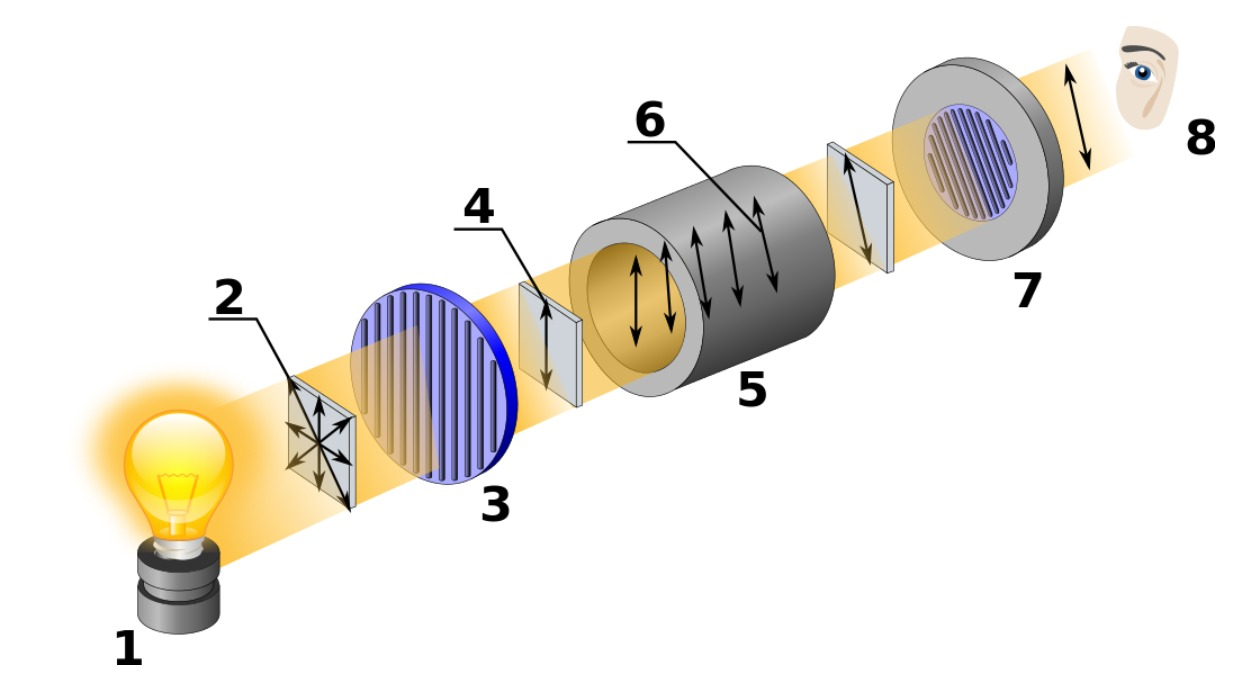
\includegraphics[width=\textwidth]{polarimeter.png}
\caption{Schematische Darstellung des Aufbaus eines Polarimeters}
\label{abb:polarimeter}
\end{figure}


\nocite{skript}

\printbibliography
\end{document}
